% !TEX program = pdflatex
% !TEX root = manuscript.tex
%Sample for icsthesis.cls
%Author: JCEPlaras
%Reminders: Omit \lipsum commands

\documentclass{icsthesis}
\usepackage{lipsum} %for generating dummy text
\usepackage{url} % break DOIs and long URLs in Literature Cited
\usepackage{xurl}
\usepackage{array}
\usepackage{longtable}

% icsthesis loads hyphenat[none]; restore breaking so lines stay inside margins
\hyphenpenalty=50
\exhyphenpenalty=50
\tolerance=2000
\emergencystretch=3em
\setlength{\hfuzz}{1pt}

%\usepackage{showframe} %for debugging the margins
                              
                              
%Replace the values here, various commands depend on this variables                                                                                                                                                            
\renewcommand{\TITLE}{AN AGENT-BASED MODEL OF LOCAL DECISION-MAKING AND DISRUPTION PROPAGATION IN THE BENGUET VEGETABLE SUPPLY CHAIN USING LARGE LANGUAGE MODELS AND A DISTILLED PLAN SELECTOR}
\renewcommand{\AUTHOR}{ACHILLES JOHN  VILLALOBOS}
\renewcommand{\DEGREE}{BACHELOR OF SCIENCE}
\renewcommand{\MAJOR}{Computer Science}
\renewcommand{\MONTH}{JANUARY}
\renewcommand{\YEAR}{2027}

\begin{document}
	
	\begin{frontmatter}
		%create title
		\maketitle
				
		\begin{approvalpage}
			The thesis hereto attached entitled \TITLE , prepared and submitted by \AUTHOR , in partial fulfillment of the requirements for the degree of \DEGREE\ (\MAJOR) is hereby accepted.
			
			\begin{multicols}{2}
				\centering
				\addsignature{ISAAC X. NEWTON}{Member, Guidance Committee} %custom command for adding signature field
				\columnbreak
				\addsignature{ISAAC X. NEWTON}{Member, Guidance Committee}
			\end{multicols}
			\addsignature{ALAN X. TURING}{Chair, Guidance Committee}
			
			Accepted in partial fulfillment of the requirements for the degree of \DEGREE\ (\MAJOR). 
			\addsignature{EDSGER W. DIJKSTRA}{Director, Institute of Graphs}
			\addsignature{STEPHEN W. HAWKING}{Dean, Graduate School\\University of the Mars Los Ba\~{n}os}
		\end{approvalpage}
		
		\begin{biosketch}
			\lipsum[4] %insert dummy text
			
			MUST NOT EXCEED ONE PAGE.		
			
			\addauthorsignaturefield
		\end{biosketch}	
		
		%acknowledgement
		\begin{acknowledgement}
			\lipsum[4]
			\lipsum[4]
			\lipsum[4]
			MUST NOT EXCEED ONE PAGE.
		\end{acknowledgement}
		
		%TOC
		\maketableofcontents
		
		%LOT
		\makelistoftables

		%LOF
		\makelistoffigures
	
		%ABSTRACT
		
		\begin{abstractwithpageno}	
		\\
		\textbf{\AUTHOR}, University of the Philippines Los Ba\~{n}os, \MONTH\ \YEAR. \textbf{\TITLE}
		\\Major Professor: PROF. EDSGER W. DIJKSTRA\\
			
			\lipsum[4]MUST NOT EXCEED ONE PAGE.
		\end{abstractwithpageno}

	\end{frontmatter}
	
	%BODY OF THESIS HERE (Use up to 3 levels only, (sec -> subsec -> subsubsec)
	\begin{mainmatter}
		\section{INTRODUCTION}

			\subsection{Background of the Study}

			Benguet supplies a large share of temperate vegetables in the Philippines. \citet{Aquino2025}, compiling Philippine Statistics Authority production for 2010--2023, report average national shares of 89.05\% for potato, 82.30\% for carrot, 66.61\% for cabbage, and 55.97\% for chayote. In 2023, Benguet accounted for 85.5\% of Cordillera vegetable output, or 361,311.6 metric tons \citep{PSARSSOCAR_nd}. Buguias accounts for about 65\% of Benguet vegetables \citep{Agoot2018}, and about 75\% of highland vegetables sold in Metro Manila originate in Benguet \citep{PNA2018}. A closure on this corridor is therefore a national temperate-vegetable problem as well as a local one.

			Cabbage, carrots, potatoes, and chayote move from highland farms through traders and trading posts into Baguio City, with a large share continuing toward downstream lowland markets. Maslan (2004), as cited in \citet{Fangasan2009}, reported the first destination of produce from Benguet and Mountain Province farms as 66.24\% to the La Trinidad Vegetable Trading Post (LTVTP), 31.76\% to Baguio Hangar Market, 3.50\% to other local Cordillera outlets, and 2\% to Region II, with about 48.9\% of farm output continuing to Greater Manila. Most recorded transactions still occur at LTVTP, even though the Benguet Agri-Pinoy Trading Center (BAPTC) is the larger facility \citep{deGuzmanBambicoBaconguis2023}. This study cites LTVTP and Hangar Market for corridor structure and simulates BAPTC, where a high-frequency posted wholesale series is available.

			The Benguet vegetable supply chain is a socio-technical system characterized by perishable produce, limited truck capacity, and distinct farmgate, wholesale, and retail price layers. Trade runs through repeated partners. \citet{deGuzmanBambicoBaconguis2023} interviewed 39 farmers and 36 traders at LTVTP, BAPTC, Hangar Market, and two private posts. In that purposive sample, 46\% of farmers named one trader, 41\% named two, and 13\% named three to five, usually disposers in a \emph{suki} arrangement often embedded in \emph{ga-it} ties (kin, friends, and people of the same ethnicity). Half of the traders named one to five \emph{suki} partners, and the rest named six or more. These sticky ties speed unloading, payment, and parking at crowded posts, while also binding farmers who owe input credit. Across the chain, farmers, traders, truckers, wholesalers, and retailers decide with incomplete or delayed information, observing a usual buyer, remaining inventory, a posted price, incomplete weather updates, or a familiar route rather than the system as a whole. In the same sample, 85\% of farmers obtained price information from local trading areas and associations rather than primarily from \emph{ga-it}. LTVTP announces a floor and ceiling twice daily, at 08:30 and 15:00, and actors verify partner talk against those postings. Under business-as-usual conditions, such locally rational decision-making sustains daily trading and price formation.

			The same mountains that support production also constrain transport. The corridor depends on four principal roads: Kennon Road, Marcos Highway, Naguilian Road, and Halsema Highway, with farm-to-market roads connecting highland production clusters to those highways. Steep cut slopes, weathered rock, and rainfall infiltration from the southwest monsoon (\emph{habagat}) and tropical cyclones cause landslides, rockfalls, and road slips. Kennon Road is the shortest Baguio--lowland link and the most frequently shut; produce trucks may still be barred even when light vehicles are allowed to pass. Halsema carries produce from Buguias, Mankayan, and Atok to the trading posts, so a cut on Halsema can delay lots past buyer windows even while the lowland outflows remain open. Similarly, a cut on a farm-to-market road can isolate a production cluster even while Halsema remains open.

			The disruption scenarios in this study are grounded in documented closures. In October 2009, Typhoon Pepeng closed Kennon Road, Marcos Highway, and Naguilian Road together, forcing vegetable trucks to queue for a reopened Marcos Highway \citep{GMANews2009}. In September 2018, after \emph{habagat} and Typhoon Ompong, erosion on Halsema increased reported travel time from Buguias to La Trinidad from about three hours to four or five hours; late trucks missed buyers, and price increases were attributed to damaged roads and intermediaries rather than empty farms \citep{PNA2018,Espiritu2018}. In July 2024, Super Typhoon Carina again rendered Kennon Road impassable \citep{Rappler2024}, and in July 2025 Kennon Road remained closed despite unofficial reports of reopening \citep{PIA2025}. In August 2026, during \emph{habagat} and tropical cyclones, a shipment of Chinese cabbage waited two days and two nights in the queue to enter the trading center before being dumped, and a shipment of carrots was only partly sold, with up to 5.8 tons discarded along Labey--Lacamen Road in Tublay \citep{AntonioDumlao2026}. Although Chinese cabbage (wombok) lies outside the modeled crop set, the carrot shipment, queue, and spoilage serve as scenario priors. Together, these events capture outflow isolation, farm-to-post delay, repeated Kennon closures, and post congestion with spoilage.

			Behavioral responses may intensify these physical shocks. Farmers may delay harvest, wait on a low posted price, or offer lots to an alternate disposer when the usual buyer is blocked. Truckers may reroute along links they believe are open or wait rather than travel. Traders may refuse lots, hold stock, or split deliveries, while wholesalers may set asks at the upper end of the posted band or ration remaining stock before spoilage. Retailers may raise prices on held inventory. Although each choice is locally rational, their interaction can convert a road disruption into delay, isolation, spoilage, price increases, and unmet demand.

			Post-event reports and official statistics document road closures, harvest variation, and price movements from farmgate to retail, but they cannot recover which local decisions produced a given shortage: who delayed harvest, cancelled trips, held inventory, or raised markups. Because those records capture only aggregate outcomes after the disruption, an agent-based model is used to study how interacting local decisions propagate shocks across this corridor.

			\subsection{Statement of the Problem}

			The overarching problem is how locally rational choices propagate a road disruption through the Benguet vegetable supply chain when actors operate with only a partial view of the system. The primary disruption experiment applies the Typhoon Ompong travel-time multiplier on Halsema (lengthening travel from about three hours to four or five hours) to a model whose monthly prices and production first match official business-as-usual records. Because a baseline fit alone cannot show how behavioral choices amplify a physical shock, amplification is measured on each outcome as the difference between a run that permits replanning and a counterfactual run that holds business-as-usual commitments fixed.

			\begin{enumerate}
				\item What constitutes business-as-usual market activity on this corridor, including farmgate, wholesale, and retail prices; Benguet production; perishability timing as a modeled constraint; and decisions made with incomplete or delayed information?
				\item Can those business-as-usual patterns be reproduced in a single agent-based model of farmers, traders, truckers, wholesalers, and retailers?
				\item When the Ompong travel-time multiplier lengthens the Halsema trip, how do delay, isolation, spoilage, price changes, and unmet demand differ between a run that permits replanning and one that holds business-as-usual intentions fixed?
				\item For each outcome sensitive to replanning, which factor changes it more relative to the baseline travel-time setting: alternate-road capacity, closure duration, the lag of the posted band and of the road advisory, trust in the official advisory, or the share of agents masked by Passive rather than Greedy response styles?
			\end{enumerate}

			\subsection{Objectives of the Study}

			The study aims to:

			\begin{enumerate}
				\item Identify the price layers, provincial production, timing constraints, and incomplete-information decisions that constitute business-as-usual corridor activity.
				\item Reproduce those business-as-usual patterns in a single agent-based model of farmers, traders, truckers, wholesalers, and retailers.
				\item Measure, under the Ompong travel-time multiplier, the difference in delay, isolation, spoilage, price changes, and unmet demand between replanning and a held commitment to business-as-usual intentions.
				\item Rank, for each outcome sensitive to replanning, the effects of alternate-road capacity, closure duration, posted-band and road-advisory lag, trust in the official advisory, and the share of agents masked by Passive rather than Greedy response styles using standardized one-factor-at-a-time contrasts followed by a crossed design on common random seeds.
			\end{enumerate}

			\subsection{Significance of the Study}

			The study provides a model for examining supply-chain disruption before a road closure occurs, rather than only after shortages materialize.

			\begin{itemize}
				\item For government agencies and local leaders (the Department of Agriculture, the Department of Public Works and Highways, and local government units along the corridor), the factor comparison identifies which physical, informational, or behavioral constraints most strongly drive each disruption outcome.
				\item For market actors (farmers, traders, truckers, and sellers), the model clarifies how interdependence across thin partner networks turns locally rational choices (such as delaying harvest, withholding stock, or raising markups) into cascading spoilage, price changes, or unmet demand.
				\item For computing and systems research, the study contributes an empirically specified agent-based model of a geographically identified highland perishable supply chain whose claims can be evaluated against public market records.
			\end{itemize}

			\subsection{Scope and Delimitation}

			The study covers the Benguet vegetable corridor, focusing on highland production clusters (especially Buguias, Mankayan, and Atok) and Baguio City markets as the primary destination inside the modeled geography. Downstream demand, including Greater Manila, enters as an aggregate load outside the cleaned road network. The four modeled crops are cabbage, carrots, potatoes, and chayote. Reyes et al. (2017), as cited in \citet{deGuzmanBambicoBaconguis2023}, list potatoes, cabbage, chayote, carrots, and wombok (Chinese cabbage) among the top Benguet commodities, with a rotation of potatoes in March--June, cabbage in July--October, and carrots in November--February; wombok is excluded from the modeled crop set. The modeled actors are farmers, traders, truckers, wholesalers, and retailers, with cooperatives entering only as information sources. Goods move along farm-to-market roads, Halsema, Kennon Road, Marcos Highway, and Naguilian Road. Trading posts serve as locations rather than decision-making agents, and BAPTC is the single simulated post because it provides the high-frequency posted wholesale series; LTVTP and Hangar Market remain cited for corridor structure and the Baguio retail sink. Farm-to-market roads in highland Benguet municipalities are included as a labeled access layer, whereas unnamed plot trails and individual farm coordinates are omitted.

			Export logistics, non-vegetable crops, national retail systems, consumer diets, and macroeconomic dynamics lie outside the study. Counterparties are synthetic usual pairs drawn from published partner-count distributions; ethnicity, kinship, and named \emph{ga-it} membership are not modeled attributes. Spoilage timing, truck capacity, and haul cost enter as structured assumptions, and named road closures serve as scenario inputs rather than a fitted calibration series.

			The primary disruption experiment tests the Ompong travel-time multiplier on Halsema without a concurrent yield shock, and the factor comparison evaluates the same shock on outcomes affected by replanning. Infrastructure factors comprise alternate-road capacity and closure duration; information factors comprise the lag of the posted band and road advisory and trust in the official advisory; and the behavioral factor varies the share of agents masked by Passive rather than Greedy styles. Both styles filter existing plans within the same five actor classes: Greedy places asks and markups at the top of the posted band and permits partner switching, whereas Passive masks partner switching and places markups at the low end of the band. Retailers do not substitute across crops.

		\section{REVIEW OF LITERATURE}

			This review examines how large language models are positioned inside agent-based and multi-agent simulations of supply chains and related socio-economic systems, focusing on symbolic or belief-desire-intention (BDI) control, structured plan selection, partner and information handling, and computational scale. As the sole reviewer, I screened 204 unique records retrieved from Web of Science and Scopus using one Boolean query, yielding a review corpus of 18 accessible full texts.

			\subsection{Conceptual Background}

			Agent-based models treat social and economic systems as populations of interacting decision makers whose local rules generate aggregate outcomes \citep{MacalNorth2010}. \citet{WooldridgeJennings1995} characterize intelligent agents as entities that perceive, deliberate, and act under incomplete information. Within that tradition, the BDI architecture of \citet{RaoGeorgeff1995} separates beliefs about the current situation, desires that encode competing goals, and intentions that commit the agent to a course of action.

			The design in this study uses that separation. An intention persists across simulation steps until it succeeds or until a drop rule removes it. Plans are drawn from a library of named alternatives, and stored trust beliefs can exclude library entries before selection among the remaining eligible plans. Without commitment and an explicit drop rule, the design reduces to reactive scripts.

			Language models can occupy different positions in that stack. Generative agents use the model as the decision maker, producing actions from prompts and memory \citep{Park2023}. A stricter arrangement stores beliefs, desires, and intentions as the control layer and restricts the language model to selecting one action from the eligible plans in that list.

			\subsection{Review Method}

			I searched Web of Science and Scopus with one string joining three conjuncts:
			\begin{quote}
			\raggedright\ttfamily\small
			("agent-based" OR "agent based" OR "multi-agent" OR BDI)\\
			AND ("large language model" OR LLM)\\
			AND ("supply chain" OR inventory OR trading).
			\end{quote}
			As of 19~September~2026, Web of Science returned 50 records and Scopus returned 191, leaving 204 unique records from 241 raw entries after DOI, EID, and title deduplication. Workshop and preprint-indexed records, including CEUR workshop papers and conference extended abstracts, entered only when they appeared in that export, without hand searching or citation chaining. A record was eligible if it used a large language model as an agent or planner inside an agent-based or multi-agent simulation of supply-chain decisions, inventory, trading, partner selection, disruption, or explicit BDI or symbolic control.

			Abstract screening accepted 19 records and excluded 185 (Figure~\ref{fig:ch2-corpus-flow}), comprising software engineering, security, or adversarial-prompting studies (21), adjacent technical domains (46), a residual class of operational dashboards and advisory systems (115), and near-duplicates (3) (Figure~\ref{fig:ch2-exclusion}). Of the 19 accepted records, 18 had accessible full texts and entered the review corpus with zero full-text exclusions; \citet{JiangJ2026b} was withdrawn from publishing and excluded without substitution. Figure~\ref{fig:ch2-corpus-dist} shows the publication year and venue distribution of the corpus, which is concentrated in 2025 and 2026 and consists primarily of conference and workshop papers.

			\begin{figure}[p]
				\centering
				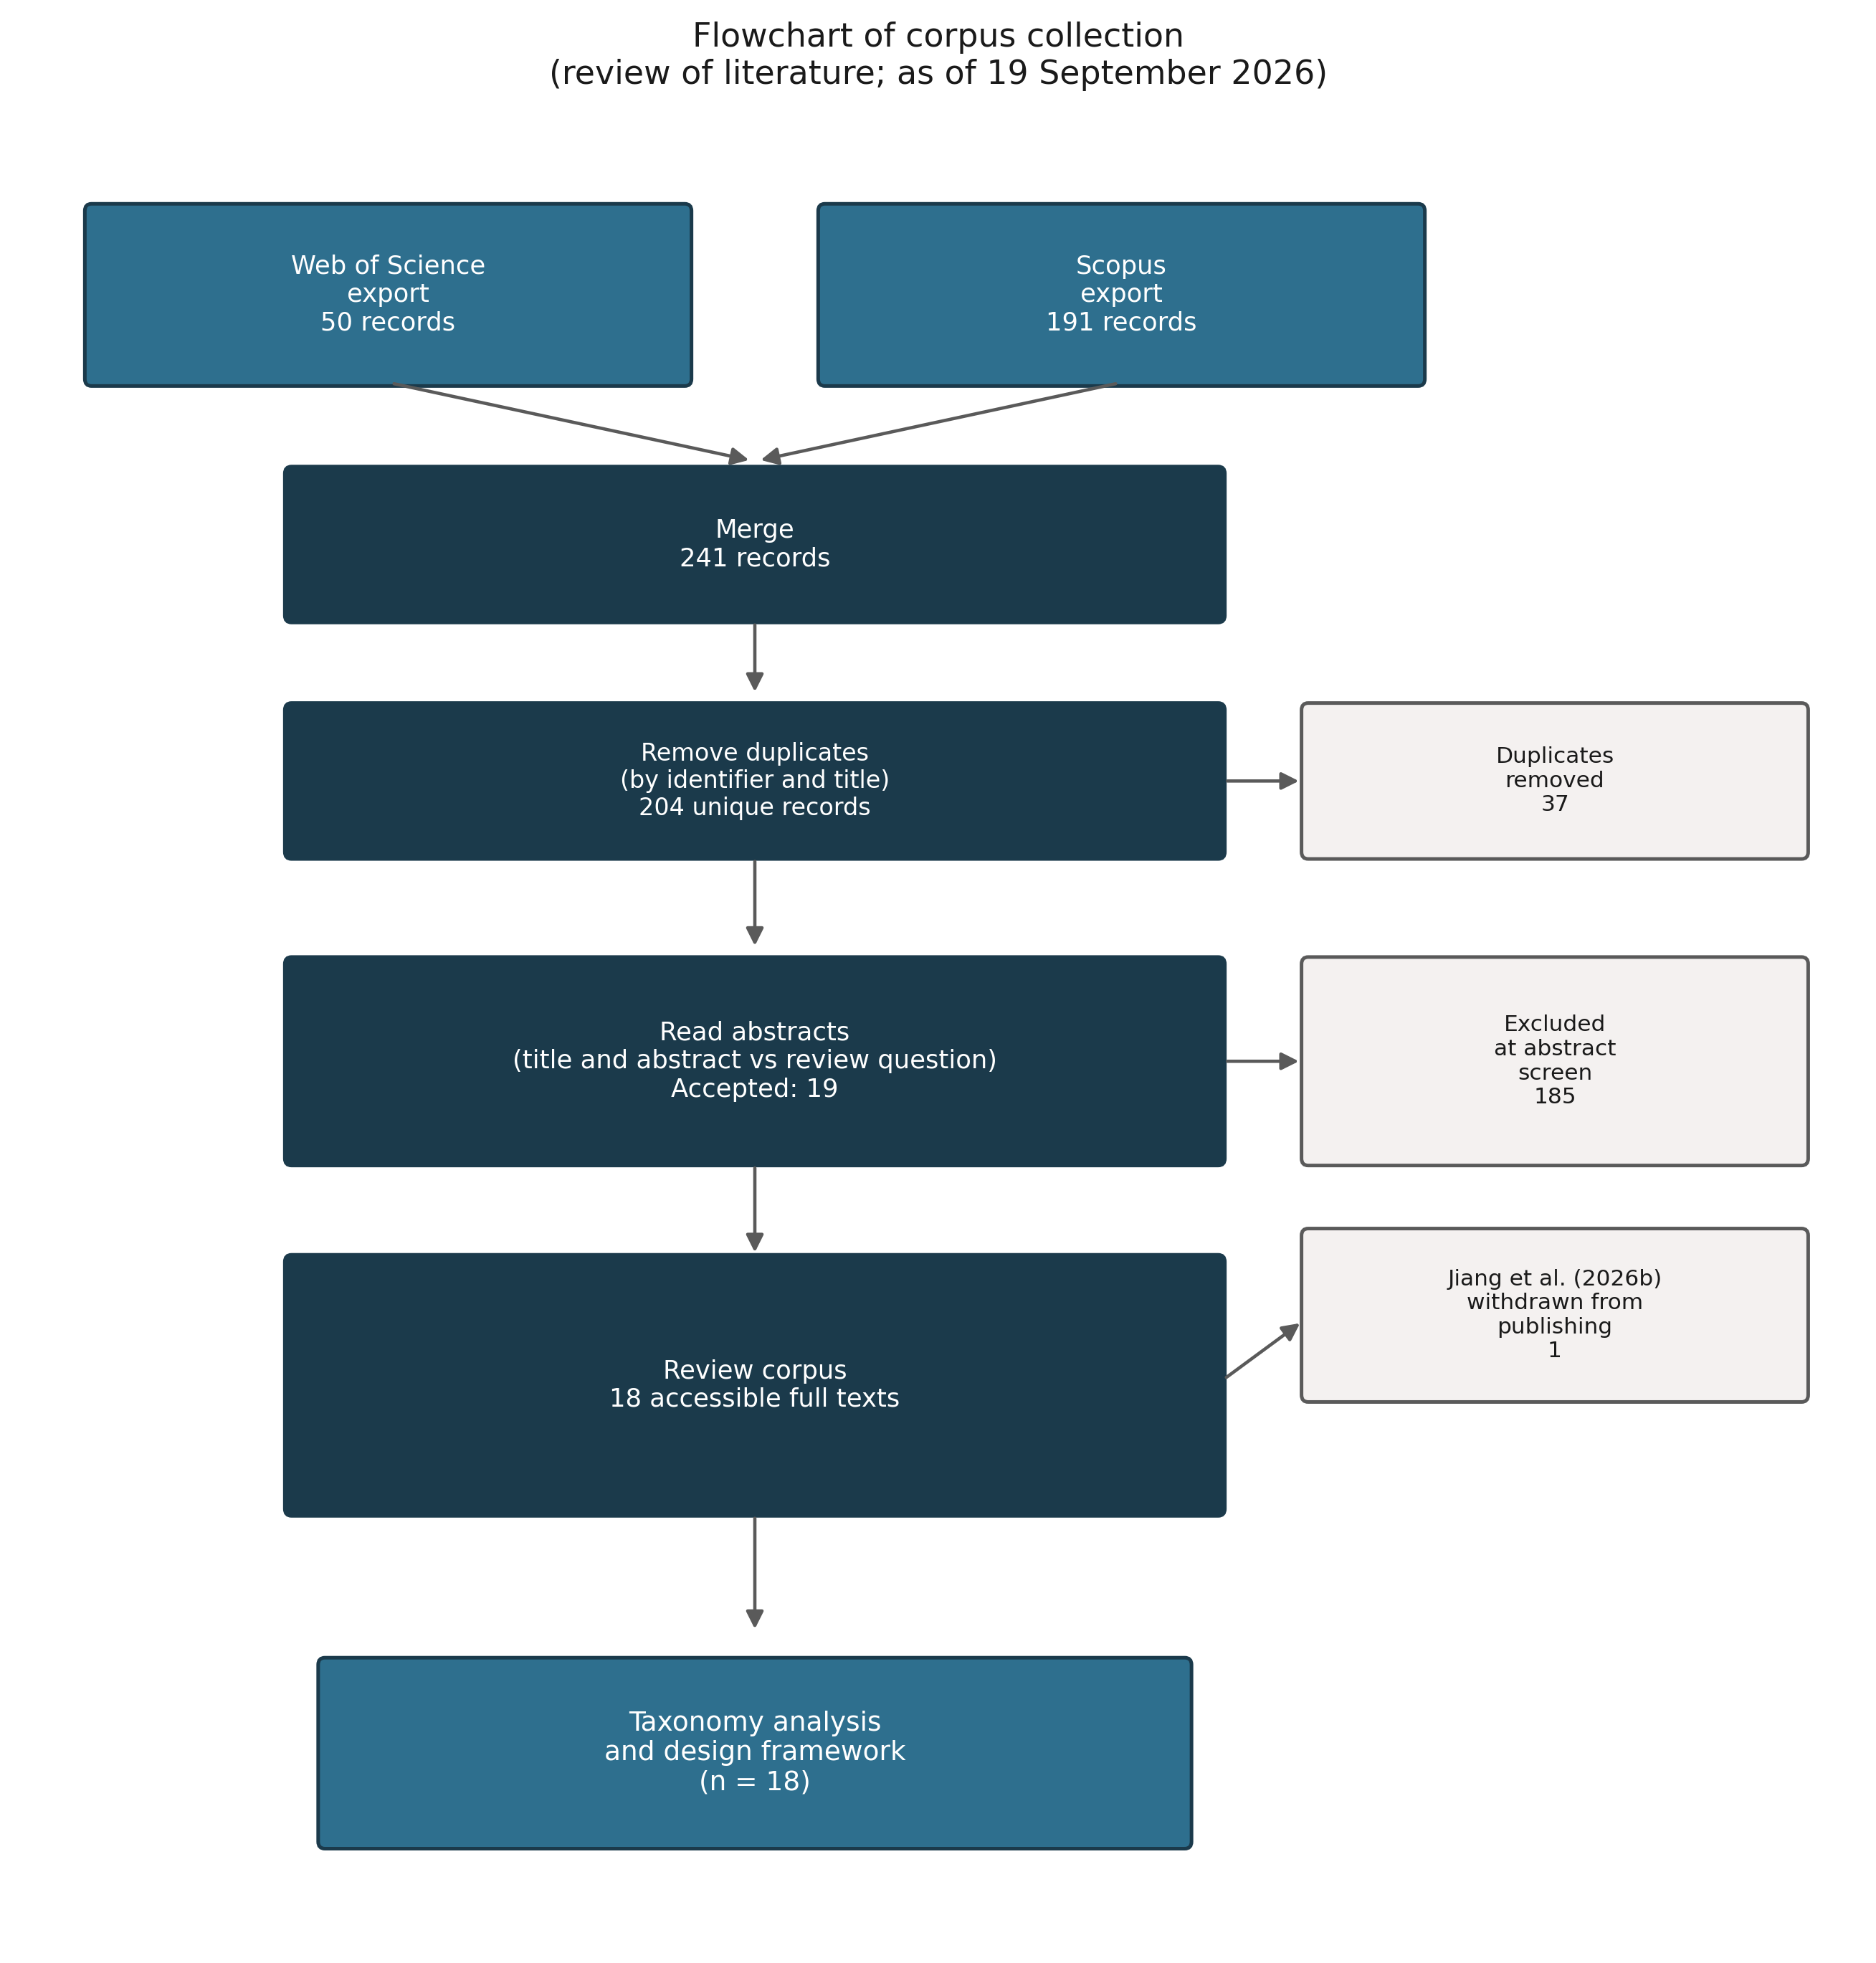
\includegraphics[width=\linewidth,height=0.82\textheight,keepaspectratio]{figures/fig1_corpus_collection}
				\caption{Review of literature: flowchart of corpus collection. Of 19 records accepted at abstract screening, 18 accessible full texts form the review corpus. One such record, \citet{JiangJ2026b}, is a paper withdrawn from publishing and is not in the review corpus.}
				\label{fig:ch2-corpus-flow}
			\end{figure}

			\begin{figure}[p]
				\centering
				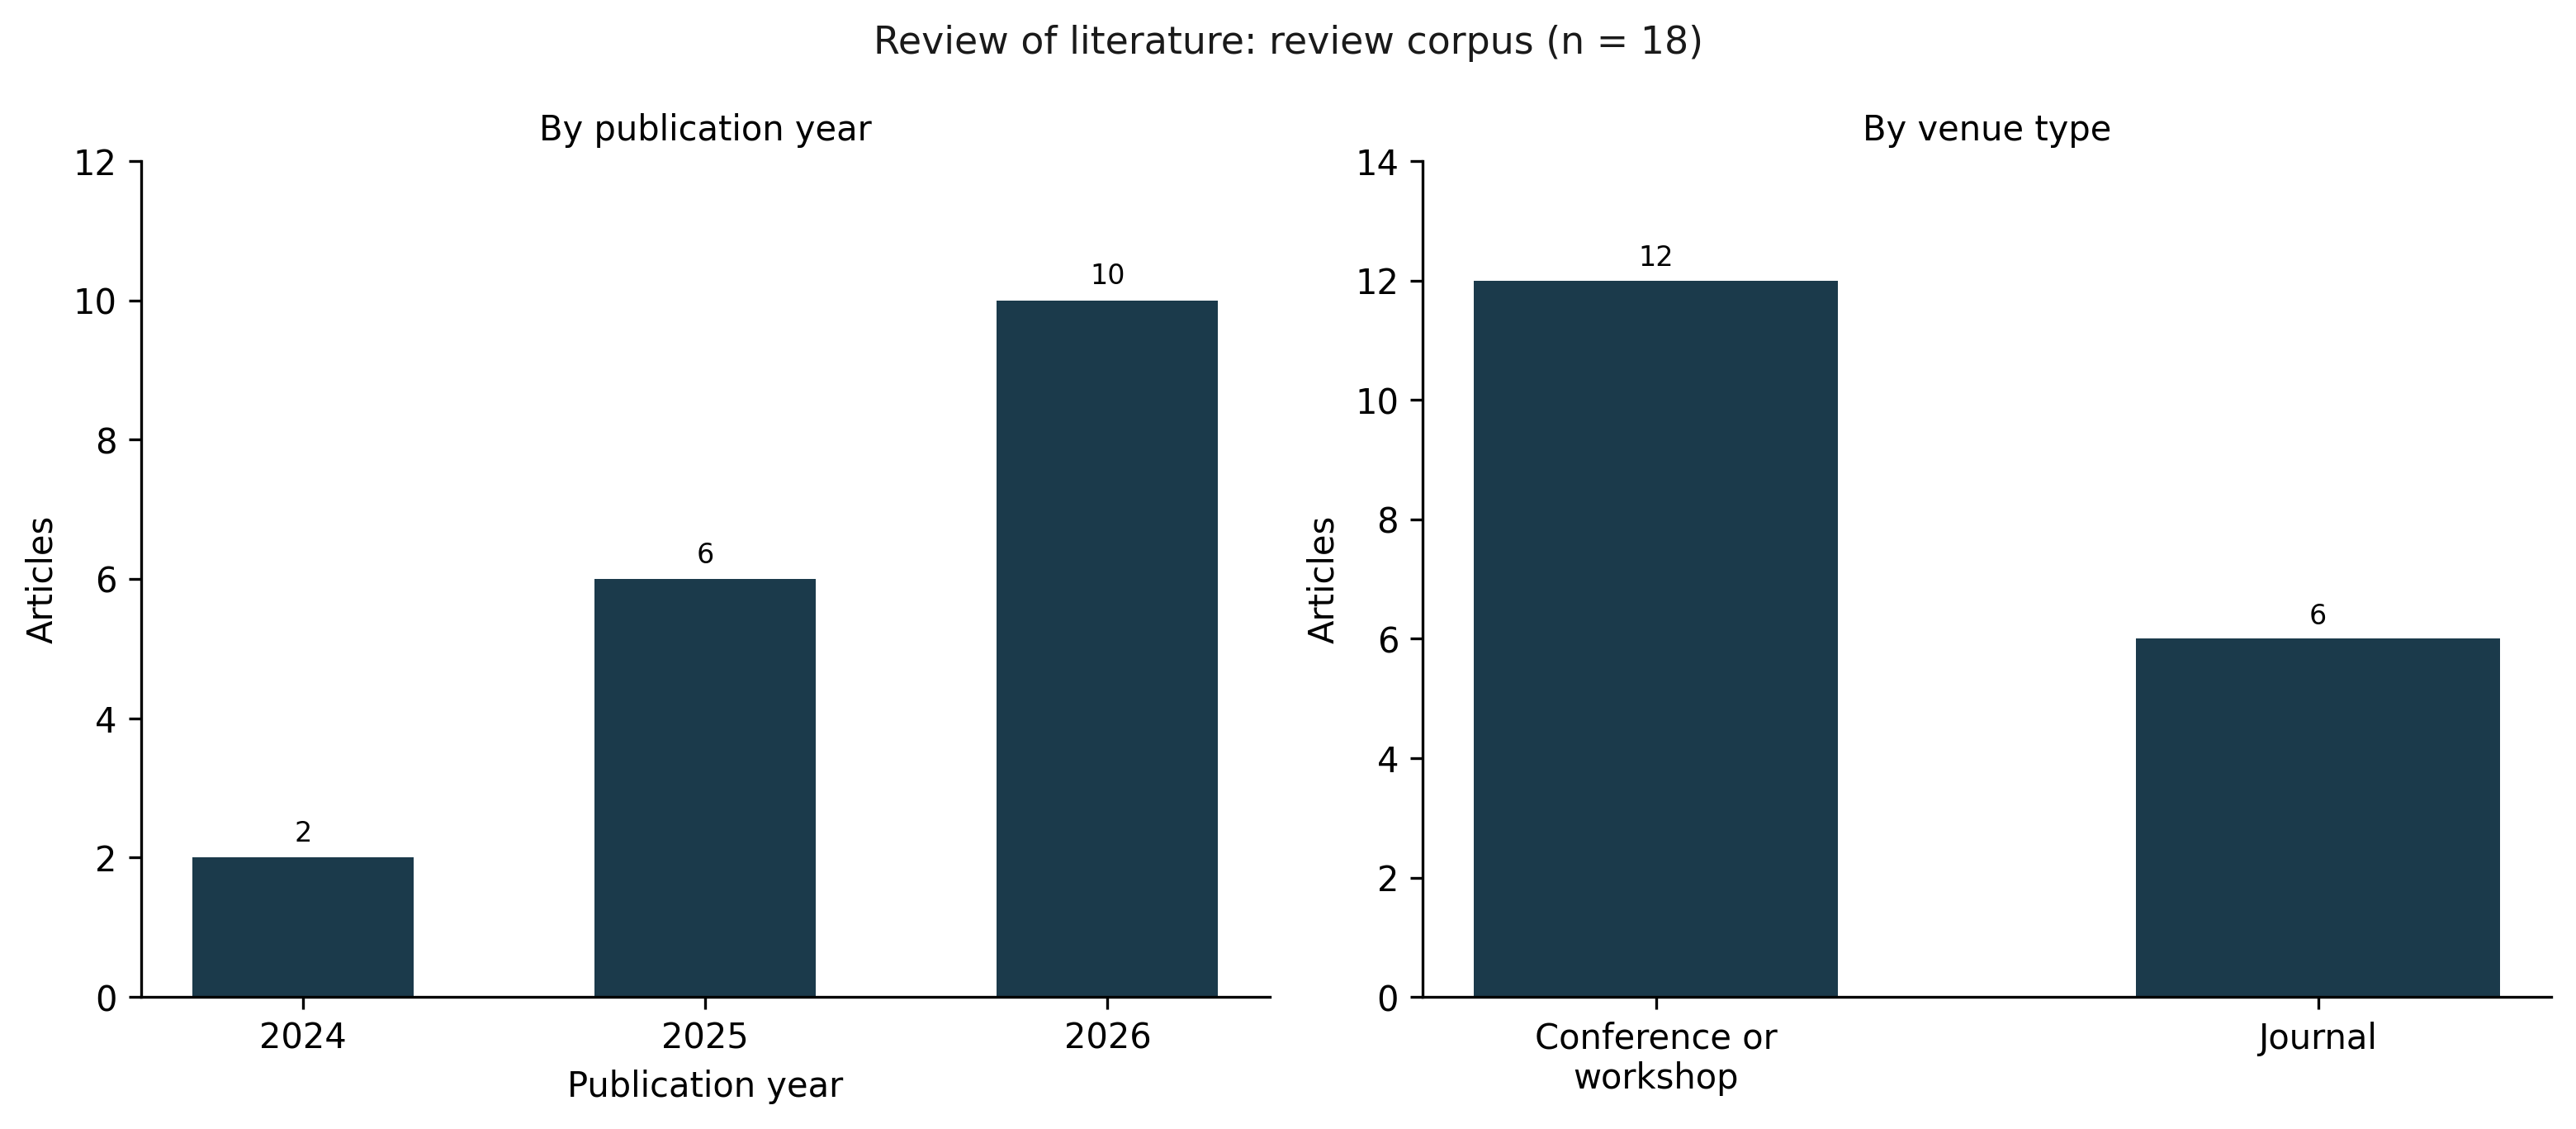
\includegraphics[width=\linewidth,height=0.82\textheight,keepaspectratio]{figures/fig2_corpus_distribution}
				\caption{Review of literature: records in the review corpus ($n = 18$), by publication year and venue type.}
				\label{fig:ch2-corpus-dist}
			\end{figure}

			\begin{figure}[p]
				\centering
				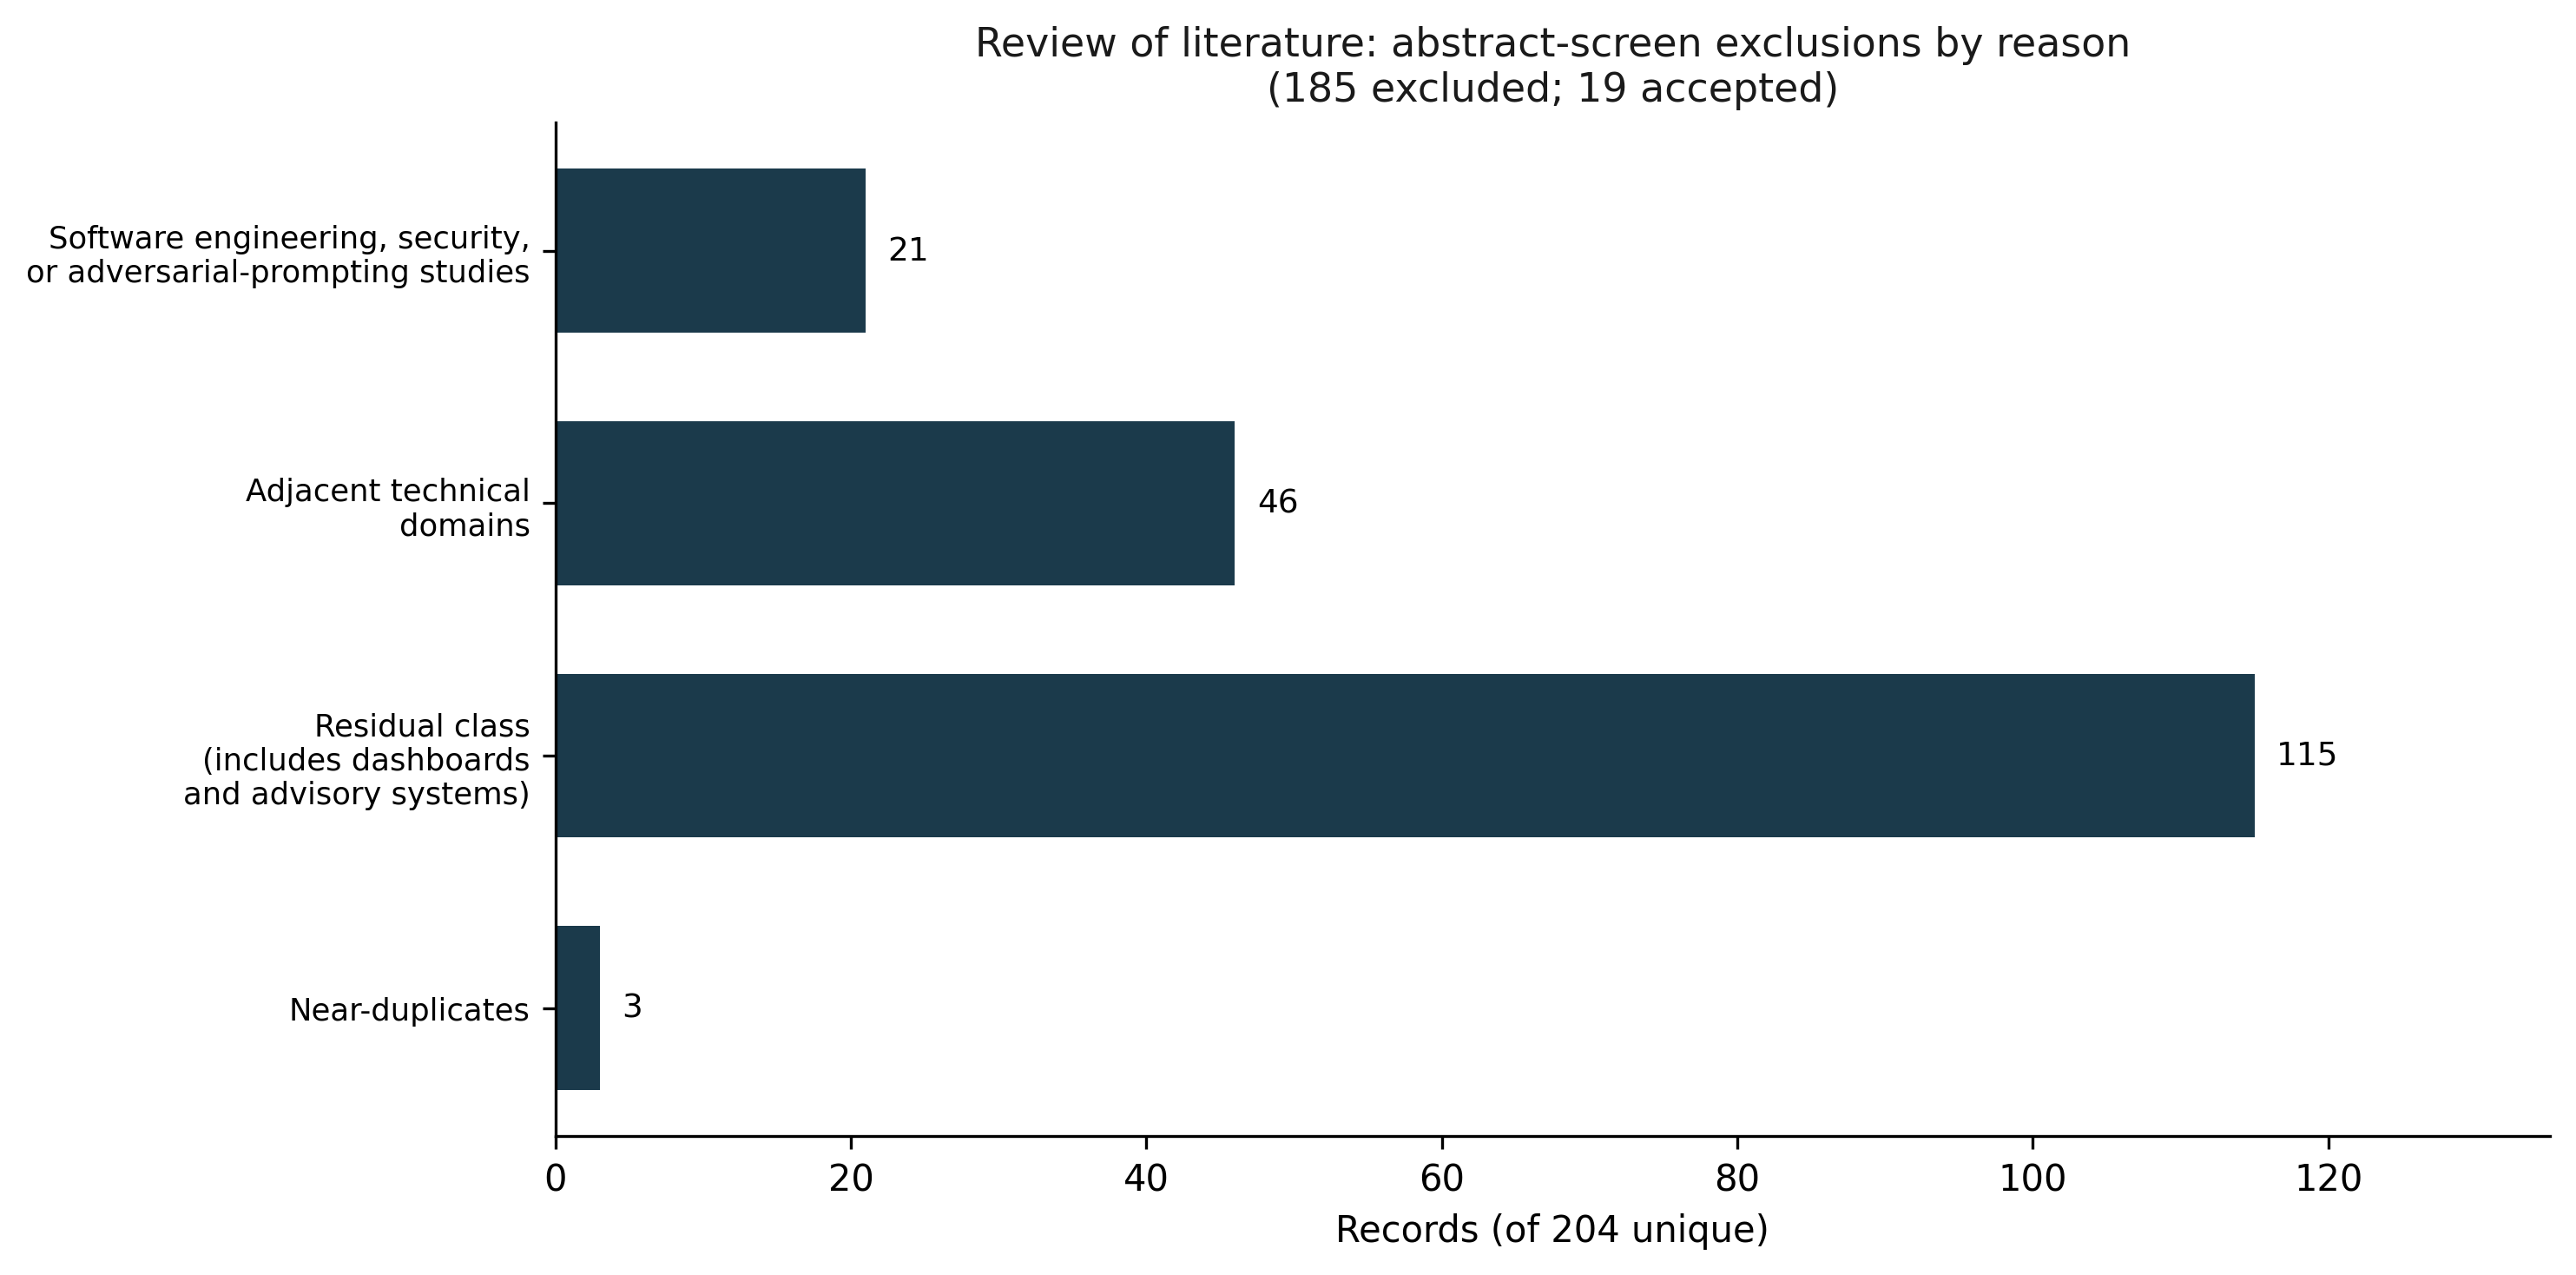
\includegraphics[width=\linewidth,height=0.82\textheight,keepaspectratio]{figures/fig5_exclusion_taxonomy}
				\caption{Review of literature: abstract-screen exclusions among 204 unique records, by reason.}
				\label{fig:ch2-exclusion}
			\end{figure}

			\clearpage

			The review corpus comprises \citet{Asaf2025}, \citet{Yoshizato2026}, \citet{Chopra2025}, \citet{Luo2026}, \citet{Gao2026}, \citet{Jannelli2025}, \citet{JiangY2026}, \citet{Kuo2026}, \citet{JiangJ2026}, \citet{VidlerWalsh2024}, \citet{Li2024}, \citet{Sowmika2026}, \citet{Phan2026}, \citet{Sashihara2025}, \citet{Zhou2026}, \citet{VidlerWalsh2025}, \citet{ParhyGoldwasser2025}, and \citet{Wang2026}. Agent design and reported evidence were extracted from the methods, implementation, and evaluation sections of each full text.

			\subsection{Design Space of Language-Model Supply-Chain Agents}

			Each full text was coded across four feature groups drawn from agent theory and the proposed architecture: language-model role, symbolic control, partner and information handling, and computational scale. A bullet marks a stated feature, and a paper may carry multiple marks in the same table; blank cells indicate features not stated in the source text.

			\begingroup
			\setstretch{1}
			\footnotesize
			\setlength{\LTcapwidth}{\textwidth}
			\setlength{\tabcolsep}{2pt}
			\renewcommand{\arraystretch}{1.12}
			\begin{longtable}[l]{@{}>{\raggedright\arraybackslash}p{0.18\textwidth}*{4}{>{\centering\arraybackslash}p{0.19\textwidth}}@{}}
			\caption{Review of literature: language-model role in the review corpus ($n = 18$). A bullet marks a stated feature. A blank cell means that feature is not stated.}
			\label{tab:ch2-role}\\
			\hline\hline
			Paper & The language model is the decision maker & The language model generates an open-ended plan & One action chosen from a named list & The language model maps data, explains a decision, or mediates a person \\
			\hline
			\endfirsthead
			\caption[]{Review of literature: language-model role in the review corpus ($n = 18$). A bullet marks a stated feature. A blank cell means that feature is not stated. (continued).}\\
			\hline\hline
			Paper & The language model is the decision maker & The language model generates an open-ended plan & One action chosen from a named list & The language model maps data, explains a decision, or mediates a person \\
			\hline
			\endhead
			\hline
			\endfoot
			\hline\hline
			\endlastfoot
			\citet{Asaf2025} &  & $\bullet$ &  &  \\
			\citet{Yoshizato2026} & $\bullet$ &  &  &  \\
			\citet{Chopra2025} & $\bullet$ &  &  &  \\
			\citet{Luo2026} & $\bullet$ &  &  &  \\
			\citet{Gao2026} & $\bullet$ &  &  & $\bullet$ \\
			\citet{Jannelli2025} & $\bullet$ &  &  &  \\
			\citet{JiangY2026} &  & $\bullet$ &  & $\bullet$ \\
			\citet{Kuo2026} & $\bullet$ &  & $\bullet$ &  \\
			\citet{JiangJ2026} & $\bullet$ &  &  &  \\
			\citet{VidlerWalsh2024} & $\bullet$ &  & $\bullet$ &  \\
			\citet{Li2024} & $\bullet$ &  &  &  \\
			\citet{Sowmika2026} & $\bullet$ &  &  &  \\
			\citet{Phan2026} & $\bullet$ &  &  & $\bullet$ \\
			\citet{Sashihara2025} & $\bullet$ &  & $\bullet$ &  \\
			\citet{Zhou2026} & $\bullet$ &  &  &  \\
			\citet{VidlerWalsh2025} & $\bullet$ &  &  &  \\
			\citet{ParhyGoldwasser2025} & $\bullet$ &  &  &  \\
			\citet{Wang2026} & $\bullet$ &  &  &  \\
			\end{longtable}
			\endgroup

			Sixteen papers mark the language model as the decision maker. Two papers, \citet{Asaf2025} and \citet{JiangY2026}, have the model generate an open-ended plan. Three papers also require one action chosen from a named list: \citet{Kuo2026}, \citet{VidlerWalsh2024}, and \citet{Sashihara2025}. Three papers mark a mapping, explanation, or mediation role, \citet{Gao2026}, \citet{JiangY2026}, and \citet{Phan2026}, in each case alongside another role. The usual arrangement in this corpus is therefore a language model used as the decision maker, with a named list appearing as a further constraint in three papers.

			\begingroup
			\setstretch{1}
			\footnotesize
			\setlength{\LTcapwidth}{\textwidth}
			\setlength{\tabcolsep}{2pt}
			\renewcommand{\arraystretch}{1.12}
			\begin{longtable}[l]{@{}>{\raggedright\arraybackslash}p{0.18\textwidth}*{3}{>{\centering\arraybackslash}p{0.26\textwidth}}@{}}
			\caption{Review of literature: symbolic control in the review corpus ($n = 18$). A bullet marks a stated feature. A blank cell means that feature is not stated.}
			\label{tab:ch2-control}\\
			\hline\hline
			Paper & Beliefs, desires, and intentions are stored across steps & Decision constraints are written in the prompt & A separate check rejects illegal or unconstrained output before execution \\
			\hline
			\endfirsthead
			\caption[]{Review of literature: symbolic control in the review corpus ($n = 18$). A bullet marks a stated feature. A blank cell means that feature is not stated. (continued).}\\
			\hline\hline
			Paper & Beliefs, desires, and intentions are stored across steps & Decision constraints are written in the prompt & A separate check rejects illegal or unconstrained output before execution \\
			\hline
			\endhead
			\hline
			\endfoot
			\hline\hline
			\endlastfoot
			\citet{Asaf2025} & $\bullet$ &  & $\bullet$ \\
			\citet{Yoshizato2026} &  & $\bullet$ &  \\
			\citet{Chopra2025} &  & $\bullet$ &  \\
			\citet{Luo2026} &  & $\bullet$ & $\bullet$ \\
			\citet{Gao2026} &  & $\bullet$ &  \\
			\citet{Jannelli2025} &  & $\bullet$ & $\bullet$ \\
			\citet{JiangY2026} &  &  & $\bullet$ \\
			\citet{Kuo2026} &  & $\bullet$ & $\bullet$ \\
			\citet{JiangJ2026} &  &  &  \\
			\citet{VidlerWalsh2024} &  & $\bullet$ &  \\
			\citet{Li2024} &  & $\bullet$ &  \\
			\citet{Sowmika2026} &  & $\bullet$ &  \\
			\citet{Phan2026} &  & $\bullet$ &  \\
			\citet{Sashihara2025} &  & $\bullet$ &  \\
			\citet{Zhou2026} &  & $\bullet$ & $\bullet$ \\
			\citet{VidlerWalsh2025} &  & $\bullet$ &  \\
			\citet{ParhyGoldwasser2025} &  & $\bullet$ &  \\
			\citet{Wang2026} &  & $\bullet$ & $\bullet$ \\
			\end{longtable}
			\endgroup

			One paper, \citet{Asaf2025}, stores beliefs, desires, and intentions across steps. Fifteen papers place decision constraints in the prompt. Seven papers describe a separate check that rejects illegal or unconstrained output before execution. Two rows need a closer reading. \citet{JiangJ2026} have no mark in Table~\ref{tab:ch2-control}. The extended abstract states chain-of-thought prompting. It does not store beliefs, desires, and intentions across steps, place a decision constraint in the prompt, or describe a separate check before an order is placed. \citet{JiangY2026} is marked for a separate check and is not marked for decision constraints written in the prompt. The language model parses policy text into a fixed schema and proposes candidate strategies. Five parses must agree on the target parameter and its direction, and two domain experts resolve a failed parse. That agreement is the separate check. State updates remain in calibrated equations, and a strategy is chosen by a softmax over mean-variance utility, so constraints written in the prompt were not assigned.

			\begingroup
			\setstretch{1}
			\footnotesize
			\setlength{\LTcapwidth}{\textwidth}
			\setlength{\tabcolsep}{2pt}
			\renewcommand{\arraystretch}{1.12}
			\begin{longtable}[l]{@{}>{\raggedright\arraybackslash}p{0.18\textwidth}*{3}{>{\centering\arraybackslash}p{0.26\textwidth}}@{}}
			\caption{Review of literature: partner and information features in the review corpus ($n = 18$). A bullet marks a stated feature. A blank cell means that feature is not stated.}
			\label{tab:ch2-partner}\\
			\hline\hline
			Paper & Partner or source scores are stored and can exclude plans & Agents share or negotiate in natural language within a period & Information is given only to a subset of firms \\
			\hline
			\endfirsthead
			\caption[]{Review of literature: partner and information features in the review corpus ($n = 18$). A bullet marks a stated feature. A blank cell means that feature is not stated. (continued).}\\
			\hline\hline
			Paper & Partner or source scores are stored and can exclude plans & Agents share or negotiate in natural language within a period & Information is given only to a subset of firms \\
			\hline
			\endhead
			\hline
			\endfoot
			\hline\hline
			\endlastfoot
			\citet{Asaf2025} &  &  &  \\
			\citet{Yoshizato2026} &  &  &  \\
			\citet{Chopra2025} &  &  &  \\
			\citet{Luo2026} &  &  &  \\
			\citet{Gao2026} &  & $\bullet$ &  \\
			\citet{Jannelli2025} &  & $\bullet$ & $\bullet$ \\
			\citet{JiangY2026} &  &  &  \\
			\citet{Kuo2026} &  &  &  \\
			\citet{JiangJ2026} &  &  & $\bullet$ \\
			\citet{VidlerWalsh2024} &  & $\bullet$ &  \\
			\citet{Li2024} &  & $\bullet$ &  \\
			\citet{Sowmika2026} &  & $\bullet$ &  \\
			\citet{Phan2026} &  & $\bullet$ &  \\
			\citet{Sashihara2025} &  &  &  \\
			\citet{Zhou2026} &  &  &  \\
			\citet{VidlerWalsh2025} &  &  &  \\
			\citet{ParhyGoldwasser2025} &  & $\bullet$ &  \\
			\citet{Wang2026} &  &  &  \\
			\end{longtable}
			\endgroup

			\begingroup
			\setstretch{1}
			\footnotesize
			\setlength{\LTcapwidth}{\textwidth}
			\setlength{\tabcolsep}{2pt}
			\renewcommand{\arraystretch}{1.12}
			\begin{longtable}[l]{@{}>{\raggedright\arraybackslash}p{0.18\textwidth}*{4}{>{\centering\arraybackslash}p{0.19\textwidth}}@{}}
			\caption{Review of literature: computational scale in the review corpus ($n = 18$). A bullet marks a stated feature. A blank cell means that feature is not stated.}
			\label{tab:ch2-scale}\\
			\hline\hline
			Paper & Each agent receives one or more language-model calls at a decision & The model is queried once for a class of agents, and each individual draws from that class & Similar stored episodes condition the next decision & A surrogate is trained on logged plan-selection decisions \\
			\hline
			\endfirsthead
			\caption[]{Review of literature: computational scale in the review corpus ($n = 18$). A bullet marks a stated feature. A blank cell means that feature is not stated. (continued).}\\
			\hline\hline
			Paper & Each agent receives one or more language-model calls at a decision & The model is queried once for a class of agents, and each individual draws from that class & Similar stored episodes condition the next decision & A surrogate is trained on logged plan-selection decisions \\
			\hline
			\endhead
			\hline
			\endfoot
			\hline\hline
			\endlastfoot
			\citet{Asaf2025} &  &  &  &  \\
			\citet{Yoshizato2026} & $\bullet$ &  & $\bullet$ &  \\
			\citet{Chopra2025} & $\bullet$ & $\bullet$ &  &  \\
			\citet{Luo2026} & $\bullet$ &  &  &  \\
			\citet{Gao2026} & $\bullet$ &  &  &  \\
			\citet{Jannelli2025} & $\bullet$ &  &  &  \\
			\citet{JiangY2026} & $\bullet$ &  &  &  \\
			\citet{Kuo2026} & $\bullet$ &  &  &  \\
			\citet{JiangJ2026} & $\bullet$ &  &  &  \\
			\citet{VidlerWalsh2024} & $\bullet$ &  &  &  \\
			\citet{Li2024} & $\bullet$ &  &  &  \\
			\citet{Sowmika2026} & $\bullet$ &  &  &  \\
			\citet{Phan2026} & $\bullet$ &  & $\bullet$ &  \\
			\citet{Sashihara2025} & $\bullet$ &  &  &  \\
			\citet{Zhou2026} & $\bullet$ &  &  &  \\
			\citet{VidlerWalsh2025} & $\bullet$ &  &  &  \\
			\citet{ParhyGoldwasser2025} & $\bullet$ &  &  &  \\
			\citet{Wang2026} & $\bullet$ &  &  &  \\
			\end{longtable}
			\endgroup

			No paper in the corpus stores partner or source scores that can exclude plans. Seven papers have agents share or negotiate in natural language within a period, and two give information only to a subset of firms. Seventeen papers make one or more language-model calls per agent at each decision, while \citet{Chopra2025} also query the model once for a class of agents. Two papers, \citet{Yoshizato2026} and \citet{Phan2026}, condition decisions on similar stored episodes, and no paper trains a surrogate on logged plan-selection decisions.

			Table~\ref{tab:ch2-corpus-profile} classifies each paper by venue (12 conference, 6 journal), domain, and decision object. Four papers receive no decision-object label under this scheme: the recycling study of \citet{Kuo2026} and the trading studies of \citet{VidlerWalsh2024}, \citet{Sashihara2025}, and \citet{ParhyGoldwasser2025}.

			\begingroup
			\setstretch{1}
			\footnotesize
			\setlength{\LTcapwidth}{\textwidth}
			\setlength{\tabcolsep}{3pt}
			\renewcommand{\arraystretch}{1.08}
			\begin{longtable}[l]{@{}>{\raggedright\arraybackslash}p{0.26\textwidth}>{\raggedright\arraybackslash}p{0.15\textwidth}>{\raggedright\arraybackslash}p{0.26\textwidth}>{\raggedright\arraybackslash}p{0.26\textwidth}@{}}
			\caption{Review of literature: venue type, domain, and decision object for the review corpus ($n = 18$). A blank decision-object cell means that none of these decision-object labels was assigned: a replenishment quantity, a firm-to-firm tie, a yes-or-no act, or a strategy written outside a named list.}
			\label{tab:ch2-corpus-profile}\\
			\hline\hline
			Paper & Venue & Domain & Decision object \\
			\hline
			\endfirsthead
			\caption[]{Review of literature: venue type, domain, and decision object for the review corpus ($n = 18$, continued). A blank decision-object cell means that none of these decision-object labels was assigned: a replenishment quantity, a firm-to-firm tie, a yes-or-no act, or a strategy written outside a named list.}\\
			\hline\hline
			Paper & Venue & Domain & Decision object \\
			\hline
			\endhead
			\hline
			\endfoot
			\hline\hline
			\endlastfoot
			\citet{Asaf2025} & Conference & eLearning & Strategy written outside a named list \\
			\citet{Yoshizato2026} & Conference & Multi-echelon replenishment & Replenishment quantity \\
			\citet{Chopra2025} & Conference & Isolate or work in an epidemic & Yes-or-no act \\
			\citet{Luo2026} & Journal & Multi-echelon replenishment & Strategy written outside a named list \\
			\citet{Gao2026} & Conference & Manufacturing firm network & Firm-to-firm tie \\
			\citet{Jannelli2025} & Journal & Multi-echelon replenishment & Replenishment quantity \\
			\citet{JiangY2026} & Journal & Mineral or policy-shock chain & Strategy written outside a named list \\
			\citet{Kuo2026} & Journal & Recycling &  \\
			\citet{JiangJ2026} & Conference & Multi-echelon replenishment & Replenishment quantity \\
			\citet{VidlerWalsh2024} & Conference & Trading or marketplace &  \\
			\citet{Li2024} & Conference & Multi-echelon replenishment & Replenishment quantity \\
			\citet{Sowmika2026} & Conference & Fashion retail replenishment & Replenishment quantity \\
			\citet{Phan2026} & Conference & Agricultural price negotiation & Strategy written outside a named list \\
			\citet{Sashihara2025} & Conference & Trading or marketplace &  \\
			\citet{Zhou2026} & Journal & Trading or marketplace & Strategy written outside a named list \\
			\citet{VidlerWalsh2025} & Conference & Trading or marketplace & Yes-or-no act \\
			\citet{ParhyGoldwasser2025} & Conference & Trading or marketplace &  \\
			\citet{Wang2026} & Journal & Coupled epidemic and economy & Strategy written outside a named list \\
			\end{longtable}
			\endgroup

			\subsection{Reported Evidence and Validation Practice}

			Table~\ref{tab:ch2-world} names the world each simulation was run on, and Table~\ref{tab:ch2-check} records model status, check, baseline, and stated limit for the 18 papers. After those tables, checks that use an observed series gathered outside the simulation are separated from checks that stay inside the run.

			\begingroup
			\setstretch{1}
			\footnotesize
			\setlength{\LTcapwidth}{\textwidth}
			\setlength{\tabcolsep}{3pt}
			\renewcommand{\arraystretch}{1.08}
			\begin{longtable}[l]{@{}>{\raggedright\arraybackslash}p{0.28\textwidth}>{\raggedright\arraybackslash}p{0.66\textwidth}@{}}
			\caption{Review of literature: the world each simulation was run on ($n = 18$).}
			\label{tab:ch2-world}\\
			\hline\hline
			Paper & World \\
			\hline
			\endfirsthead
			\caption[]{Review of literature: the world each simulation was run on ($n = 18$). (continued).}\\
			\hline\hline
			Paper & World \\
			\hline
			\endhead
			\hline
			\endfoot
			\hline\hline
			\endlastfoot
			\citet{Asaf2025} & Java eLearning prototype for one self-directed learner \\
			\citet{Yoshizato2026} & Synthetic multi-echelon inventory scenarios \\
			\citet{Chopra2025} & Census-based New York City population with BLS and CDC series \\
			\citet{Luo2026} & Synthetic Sema-Sim supply-chain benchmark \\
			\citet{Gao2026} & Paper-packaging firm network, eight quarters in 2023--2024 \\
			\citet{Jannelli2025} & Synthetic Merton jump-diffusion demand \\
			\citet{JiangY2026} & Historical nickel series for backcast; quarterly scenarios 2025--2035 \\
			\citet{Kuo2026} & Synthetic NetLogo recycling world \\
			\citet{JiangJ2026} & Synthetic Beer Game \\
			\citet{VidlerWalsh2024} & Synthetic bilateral gilt-trading prompts \\
			\citet{Li2024} & One Amazon product's daily sales for one year \\
			\citet{Sowmika2026} & Synthetic four-outlet fashion simulation \\
			\citet{Phan2026} & Agri Sung transaction logs and 30 buyer transcripts \\
			\citet{Sashihara2025} & Synthetic marketplace, checked against Ocean Protocol transactions \\
			\citet{Zhou2026} & Synthetic six-agent electricity-carbon market \\
			\citet{VidlerWalsh2025} & Synthetic gilt market; client cash and bonds drawn log-normal, with an APRA pension-size illustration \\
			\citet{ParhyGoldwasser2025} & Technology-sector prices from Polygon and news from Marketaux, over six months \\
			\citet{Wang2026} & Synthetic population of 50, initialized from census-style and World Bank distributions \\
			\end{longtable}
			\endgroup

			\begingroup
			\setstretch{1}
			\footnotesize
			\setlength{\LTcapwidth}{\textwidth}
			\setlength{\tabcolsep}{3pt}
			\renewcommand{\arraystretch}{1.08}
			\begin{longtable}[l]{@{}>{\raggedright\arraybackslash}p{0.15\textwidth}>{\raggedright\arraybackslash}p{0.13\textwidth}>{\raggedright\arraybackslash}p{0.24\textwidth}>{\raggedright\arraybackslash}p{0.21\textwidth}>{\raggedright\arraybackslash}p{0.20\textwidth}@{}}
			\caption{Review of literature: model status, check, baseline, and stated limit ($n = 18$).}
			\label{tab:ch2-check}\\
			\hline\hline
			Paper & Model status & Check & Baseline & Stated limit \\
			\hline
			\endfirsthead
			\caption[]{Review of literature: model status, check, baseline, and stated limit ($n = 18$, continued).}\\
			\hline\hline
			Paper & Model status & Check & Baseline & Stated limit \\
			\hline
			\endhead
			\hline
			\endfoot
			\hline\hline
			\endlastfoot
			\citet{Asaf2025} & Not stated & Prototype latency: session initialization under 5 seconds, belief update under 100 ms, agent response 2--5 seconds, and plan generation 2--4 minutes (Table 2) & Not stated & The authors state that the implementation remains limited in scope and that a comparison with classical BDI agents and language-model agents on established benchmarks is future work (Section 5). \\
			\citet{Yoshizato2026} & No training run stated & Relative gap to the optimal value, delta = absolute value of (Opt minus r) divided by Opt, averaged over five episodes (Table 1) & The optimal value, plus InvAgent variants, base-stock, tracking-demand, IPPO, and MAPPO (Section 3) & The authors state that the safety-stock prompt degrades under time-varying demand (Section 3). \\
			\citet{Chopra2025} & No training run stated & Mean-square error on a later infection window (16 weeks) and unemployment window (80 weeks), Table 1: archetype 95.17 (SD 20.23) and 24.59 (SD 1.5); heuristic 2914.73 (SD 300.25) and 41.05 (SD 0.1); per-person language-model agents 4311.70 (SD 674.14) and 56.98 (SD 2.5). Section 5 also reports correlation of archetype work attendance with Bureau of Labor Statistics participation. & Hand-crafted heuristic agents at full population scale, and per-person language-model agents limited to 300 queries per step and then scaled; Section 5 also uses observed Bureau of Labor Statistics participation & The authors state that performance is measured against mesoscopic census data and macroscopic forecasts, and that data contamination and biased outputs remain open problems (Section 8). \\
			\citet{Luo2026} & No training run stated & Semantic Fidelity Index, a weighted sum of constraint alignment, one minus a reinterpretation score, trajectory consistency, and a violation penalty (Section 6). Table 4 reports ReflectiChain at 88.7, ReflAct at 87.8, and ReAct at 84.4, with drift coefficient alpha 0.823 for ReflectiChain. & Six other prompting strategies on Sema-Sim: NoThinking, chain-of-thought, ReAct, self-consistency, ReflAct, and Reflexion (Section 7.2) & The authors state that rationale text may not match the decision process, that Sema-Sim is supply-chain only, and that an end-to-end trained world model is future work (Section 10). \\
			\citet{Gao2026} & No training run stated & Next-quarter partner-edge accuracy, precision, recall, and F1 against the observed network, plus Gwet's AC1 on add, remove, or keep decisions (Section 5.1, Table 1). A separate 5-point Likert questionnaire covers workload, usability, and effectiveness with 12 participants (Section 7). & Observed partner edges at the next quarter (Section 5.1). The user study states that no baseline system was compared (Section 8.4.1). & The authors state that the user study was a short laboratory session without a baseline system, and that the dataset is a small paper-products sample (Section 8.4). \\
			\citet{Jannelli2025} & No training run stated & Global supply-chain cost, and bullwhip as a coefficient of variation (Table 2). Negotiation versus information sharing with the EOQ tool is reported as a 66.2 percent bullwhip reduction for Gemini Pro and 33.2 percent for Gemini Flash. & An (S, s) policy with S = 100 and s = 60; a tool-only agent; and, for bullwhip, the centralized-demand calculation reported in Section 5.1 & The authors state that the study uses only Gemini models and that prompts were manually engineered, with the smaller model as the optimization target (Section 8). \\
			\citet{JiangY2026} & No training run stated & Backcast price MAPE on the 2022 LME short squeeze, 12.3 percent versus 28.6 percent for the rule-based model, described as 57 percent lower error; export-ban production response error for the 2020 Indonesian ore ban, 8.6 percent versus 18.2 percent, described as 53 percent lower error (Table 5 and Section 4) & A rule-based agent-based model with the same equations, data, seed, and Monte Carlo design, and with hard-coded threshold rules in place of language-model parsing and softmax selection (Section 4) & The authors state that the forward scores are conditional stress tests, that firm microdata are incomplete, and that domain-tuned language models are future work (Section 5). \\
			\citet{Kuo2026} & No training run stated & Recycling rate, mean 90.04 percent (SD 2.10) under the rule-based model and 94.53 percent (SD 1.75) under GPT-4o, p less than 0.001, Cohen's d = 1.78, from 30 replications (Section 4.2) & Deterministic IF-THEN rules in NetLogo, 30 replications (Section 4.1) & The authors state that the results are conditional on one prompt, that a GPT-only versus GPT-plus-retrieval ablation was not run, and that no external dataset was used (Sections 3.4 and 5; data-availability note). \\
			\citet{JiangJ2026} & No training run stated & Order variance, compared with one-tailed Mann-Whitney U tests across information regimes and model families (Section 3 and Table 1) & Other model families under the same information regimes, and hybrid teams against a pure Qwen society (Figure 1 and Table 1) & Not stated \\
			\citet{VidlerWalsh2024} & No training run stated & Share of 300 simulations selecting the prompted no-trade action, 180 of 300 (60 percent); share of 300 simulations with an executed trade, 5.7 percent, set beside a cited 2024 U.S. equity order-to-trade ratio of about 4.61 percent (Section III) & The prompted no-trade premise in the first test. The second test cites a U.S. equity order-to-trade ratio and states that a direct human-frequency comparison is absent (Section III). & The authors present the runs as a proof of concept, state that prompt design was opportunistic, and report that both initial holdings were recovered in 2.34 percent of responses (Sections III and IV). \\
			\citet{Li2024} & No training run stated & Inventory turnover, stockout rate, shipping fees, holding fees, and total cost against the firm's recorded figures (Table 6): simulation turnover 33.82 versus recorded 23.77; stockout 0.00 percent in both; total cost 1699.53 dollars versus 2160.21 dollars & The same product's recorded inventory outcomes (Table 6) & The authors state that manufacturing and shipping delays were not modeled, and that the forecasting agent required several retries before it produced a usable model (Discussion). \\
			\citet{Sowmika2026} & No training run stated & Replenishment volume under named events versus normal-operation periods (Figure 5), and minimum outlet inventory, reported as not below 180 units over 100 steps (Section VI.B) & Normal-operation periods in the same simulation (Figure 5). No external method is named. & The authors state that multi-turn reasoning latency is a constraint for high-frequency logistics, while judging it acceptable for a daily cycle (Section VII.C). \\
			\citet{Phan2026} & No training run stated & Deal success rate, wins divided by scenarios, 25 of 30 (83.33 percent), and target-to-actual price gap, the mean of final price over target price minus 1, reported as -1.7556 percent (Section 4.2). Price models are also scored with MAE, RMSE, R-squared, and MAPE on transaction logs (Table 1). & Ablations that remove the manager, the receiver modules, or the cost estimator (Table 2), and six other regressors on the transaction logs (Table 1) & The authors name larger product portfolios and stronger human supervision as future work (Section 5). \\
			\citet{Sashihara2025} & Not stated & Power-law exponent and Kolmogorov-Smirnov distance for purchases per dataset, 2.58 and 0.067 in the simulation versus 2.30 and 0.0259 in Ocean Protocol, plus four other distributional metrics rated in Table IV & Ocean Protocol Datatoken transactions, 6,826 records from 30 May 2022 to 20 June 2025 (Section IV.C) & The authors state that a 40-step horizon and a six-action buyer list limited heavy-buyer frequency, and that three of the five metrics diverged from the Ocean Protocol series (Section VI). \\
			\citet{Zhou2026} & No training run stated & Annual profit and annual emissions against Q-learning: 1.999 times 10 to the 9 CNY and 6597 ktCO2, versus 1.558 times 10 to the 9 CNY and 7759 ktCO2, described as a 28.3 percent profit increase and a 15.0 percent emission reduction (Section V.B) & Q-learning with 160 states, 12 discrete bid actions, and 1000 training rounds (Section V.B) & The authors state that distillation of frequent subtasks into lightweight policy models, and domain-adaptive fine-tuning, are future work, and that the case is a simplified verification market (Sections V.A and VI.B). \\
			\citet{VidlerWalsh2025} & No training run stated & Share of client trade-now answers. With an aversion prompt, 0 of more than 2800 requests agreed to trade, across 200 societies (Section 4.2). In the later yes-or-no setting, 56.9 percent of calls answered yes (Section 4.3). & The same TRIBE market with a Bernoulli trade desire and no language-model call, 200 societies, mean maximum life 1136 steps (Section 4.1 and Table 2) & The authors state that prompts were tested opportunistically and that they do not assign a cause to the aversion result (Sections 2 and 4.2). \\
			\citet{ParhyGoldwasser2025} & No training run stated & Persona-alignment tests, 20 increasing-risk cases and 20 increasing-opportunity cases, and portfolio paths from a 100,000 dollar start over three runs; collaboration profit is compared across incentive rules (Section IV). No numeric portfolio value is stated in the text. & Agents without personas, solo traders, and a consensus-bonus rule versus an influence bonus (Section IV) & The authors state that the 3B LLaMA model, the six-month simplified market, and the lack of live trading limit the result (Limitations). \\
			\citet{Wang2026} & No training run stated & Time from a comparable initial state to the infection peak in the unmitigated scenario: simulation tick 284, stated as 11.83 days, set beside a China CDC span of about 12 days from 12 January 2020 to the 24 January 2020 peak (Section 5.5) & China CDC daily new cases for the early 2020 outbreak, from a report of 72,314 cases (Section 5.5). Scenario A is also the reference for the sensitivity plots. & The authors state that contact networks and supply chains are simplified, that vaccination and reinfection are omitted, and that a language-model call per agent blocks direct expansion beyond 10,000 persons (Section 7.1). \\
			\end{longtable}
			\endgroup

			Across the corpus, every paper names a simulated world and an evaluation check (Tables~\ref{tab:ch2-world} and~\ref{tab:ch2-check}). Seventeen papers name a baseline (all except \citealp{Asaf2025}), sixteen use a pretrained model without fine-tuning, and model training status is not stated for two papers.

			Seven papers evaluate results against an external observed record such as a time series, transaction log, or observed network: \citet{Chopra2025}, \citet{Gao2026}, \citet{JiangY2026}, \citet{Li2024}, \citet{Phan2026}, \citet{Sashihara2025}, and \citet{Wang2026}. Synthetic scenarios, within-run contrasts, and cited ratios that authors decline to treat as direct comparisons are excluded from this count.

			\subsection{Gaps Relative to the Proposed Architecture}

			Four features of the architecture proposed in this study were coded during extraction: selection of one action from a named list inside stored beliefs, desires, and intentions; a drop rule for a committed intention; stored partner or source scores that can exclude plans; and a surrogate trained on logged plan-selection decisions. None of the 18 papers implements all four features together, and each feature is absent from the corpus as coded here.

			The corpus contains no supply-chain model that selects one action from a named list inside persistent beliefs, desires, and intentions. \citet{Asaf2025} maintain fuzzy beliefs, desires, and intentions, but the language model generates an open-ended plan in an eLearning prototype. No paper states a post-commitment drop rule for an intention; \citet{Zhou2026} reject or scale illegal bids before market clearing, which checks bid validity rather than dropping a committed plan. No paper stores a partner or source score and uses it to remove plans before selection. \citet{Kuo2026} keep a recycler's reputation in the prompt. That score does not remove plans from a fixed list before the model is called. A separate check can still reject the output before the action runs. Finally, no paper trains a surrogate on logged plan-selection decisions, although \citet{Zhou2026} identify subtask distillation into lightweight policy models as future work.

			\subsection{Implications for the Present Study}

			This study combines those four features for the Benguet vegetable corridor, using logged plan-selection decisions to train a lightweight surrogate for Monte Carlo execution with gradient-boosted trees as a tabular baseline \citep{Grinsztajn2022}. Corridor structure and prices draw on \citet{deGuzmanBambicoBaconguis2023} and the BAPTC posted wholesale series \citep{AgriTrakPH2025}, while disruption scenarios derive from the documented road closures in Chapter~1.

			Repeated disruption runs cannot ask the model for every agent at every decision. One query for a whole role would drop each agent's partner score and current intention. A lookup of similar past episodes still asks the model at every decision. The logged decisions train a small model that selects the plan in those runs, using the same beliefs, desires, and intentions.

			These corpus absences apply strictly to the 18 accessible papers retrieved from Web of Science and Scopus as of 19~September~2026 without hand searching; relevant work outside those databases or indexed without the query terms would not appear in the 204 records, and the corpus is predominantly 2025--2026 conference and workshop proceedings (Figure~\ref{fig:ch2-corpus-dist}). Table~\ref{tab:ch2-alignment} maps each architectural feature to its corresponding corridor mechanism from Chapter~1.

			\begingroup
			\setstretch{1}
			\footnotesize
			\setlength{\LTcapwidth}{\textwidth}
			\setlength{\tabcolsep}{3pt}
			\renewcommand{\arraystretch}{1.12}
			\begin{longtable}[l]{@{}>{\raggedright\arraybackslash}p{0.36\textwidth}>{\raggedright\arraybackslash}p{0.58\textwidth}@{}}
			\caption{Review of literature: alignment between the four features in the proposed design and the corridor mechanisms stated in Chapter~1.}
			\label{tab:ch2-alignment}\\
			\hline\hline
			Feature already in the design & Corridor mechanism already in Chapter~1 \\
			\hline
			\endfirsthead
			\caption[]{Review of literature: alignment between the four features in the proposed design and the corridor mechanisms stated in Chapter~1 (continued).}\\
			\hline\hline
			Feature already in the design & Corridor mechanism already in Chapter~1 \\
			\hline
			\endhead
			\hline
			\endfoot
			\hline\hline
			\endlastfoot
			One action from a named list inside beliefs, desires, and intentions that persist & Local choices under a partial view: delay harvest, sell to the usual disposer, reroute, hold, or raise a markup. Official series cannot recover those choices. \\
			A drop rule after commitment & A plan continues until success, failure, or an explicit drop, including a confirmed closure, a trust threshold, or spoilage pressure. \\
			Stored partner or source scores that can exclude plans & Repeated \emph{suki} partners, and price or road signals that conflict across the posted band, an official advisory, and the last transaction with a partner. \\
			A surrogate trained on logged decisions & Repeated disruption runs after business as usual is matched, without a live language-model call on every step. \\
			\end{longtable}
			\endgroup

	\section{METHODOLOGY}

			The modeling pipeline proceeds in three stages: assembling empirical data and a conceptual model, constructing the simulation world and decision architecture, and calibrating business as usual before evaluating disruption scenarios (Figure~\ref{fig:ch3-workflow}; Table~\ref{tab:ch3-workflow}).

			The conceptual model follows the PARDI method \citep{Etienne2016}, which organizes a socio-technical system by its problematic situation, actors, resources, dynamics, and interactions. PARDI descends from ARDI, a participatory co-construction method in natural-resources management \citep{Etienne2011}. Because no stakeholder workshop was held, I constructed the conceptual model from the corridor records in Chapter~1, the frozen datasets, and the trading-structure evidence of \citet{deGuzmanBambicoBaconguis2023}.

			Agent decisions operate within a belief-desire-intention (BDI) architecture \citep{RaoGeorgeff1995} equipped with stored trust scores and a fixed plan library. A large language model acts as a plan-selection teacher on residual decisions, and logged teacher choices train a distilled selector for Monte Carlo runs.

		\subsection{Study Workflow}

			\begin{figure}[htbp]
				\centering
				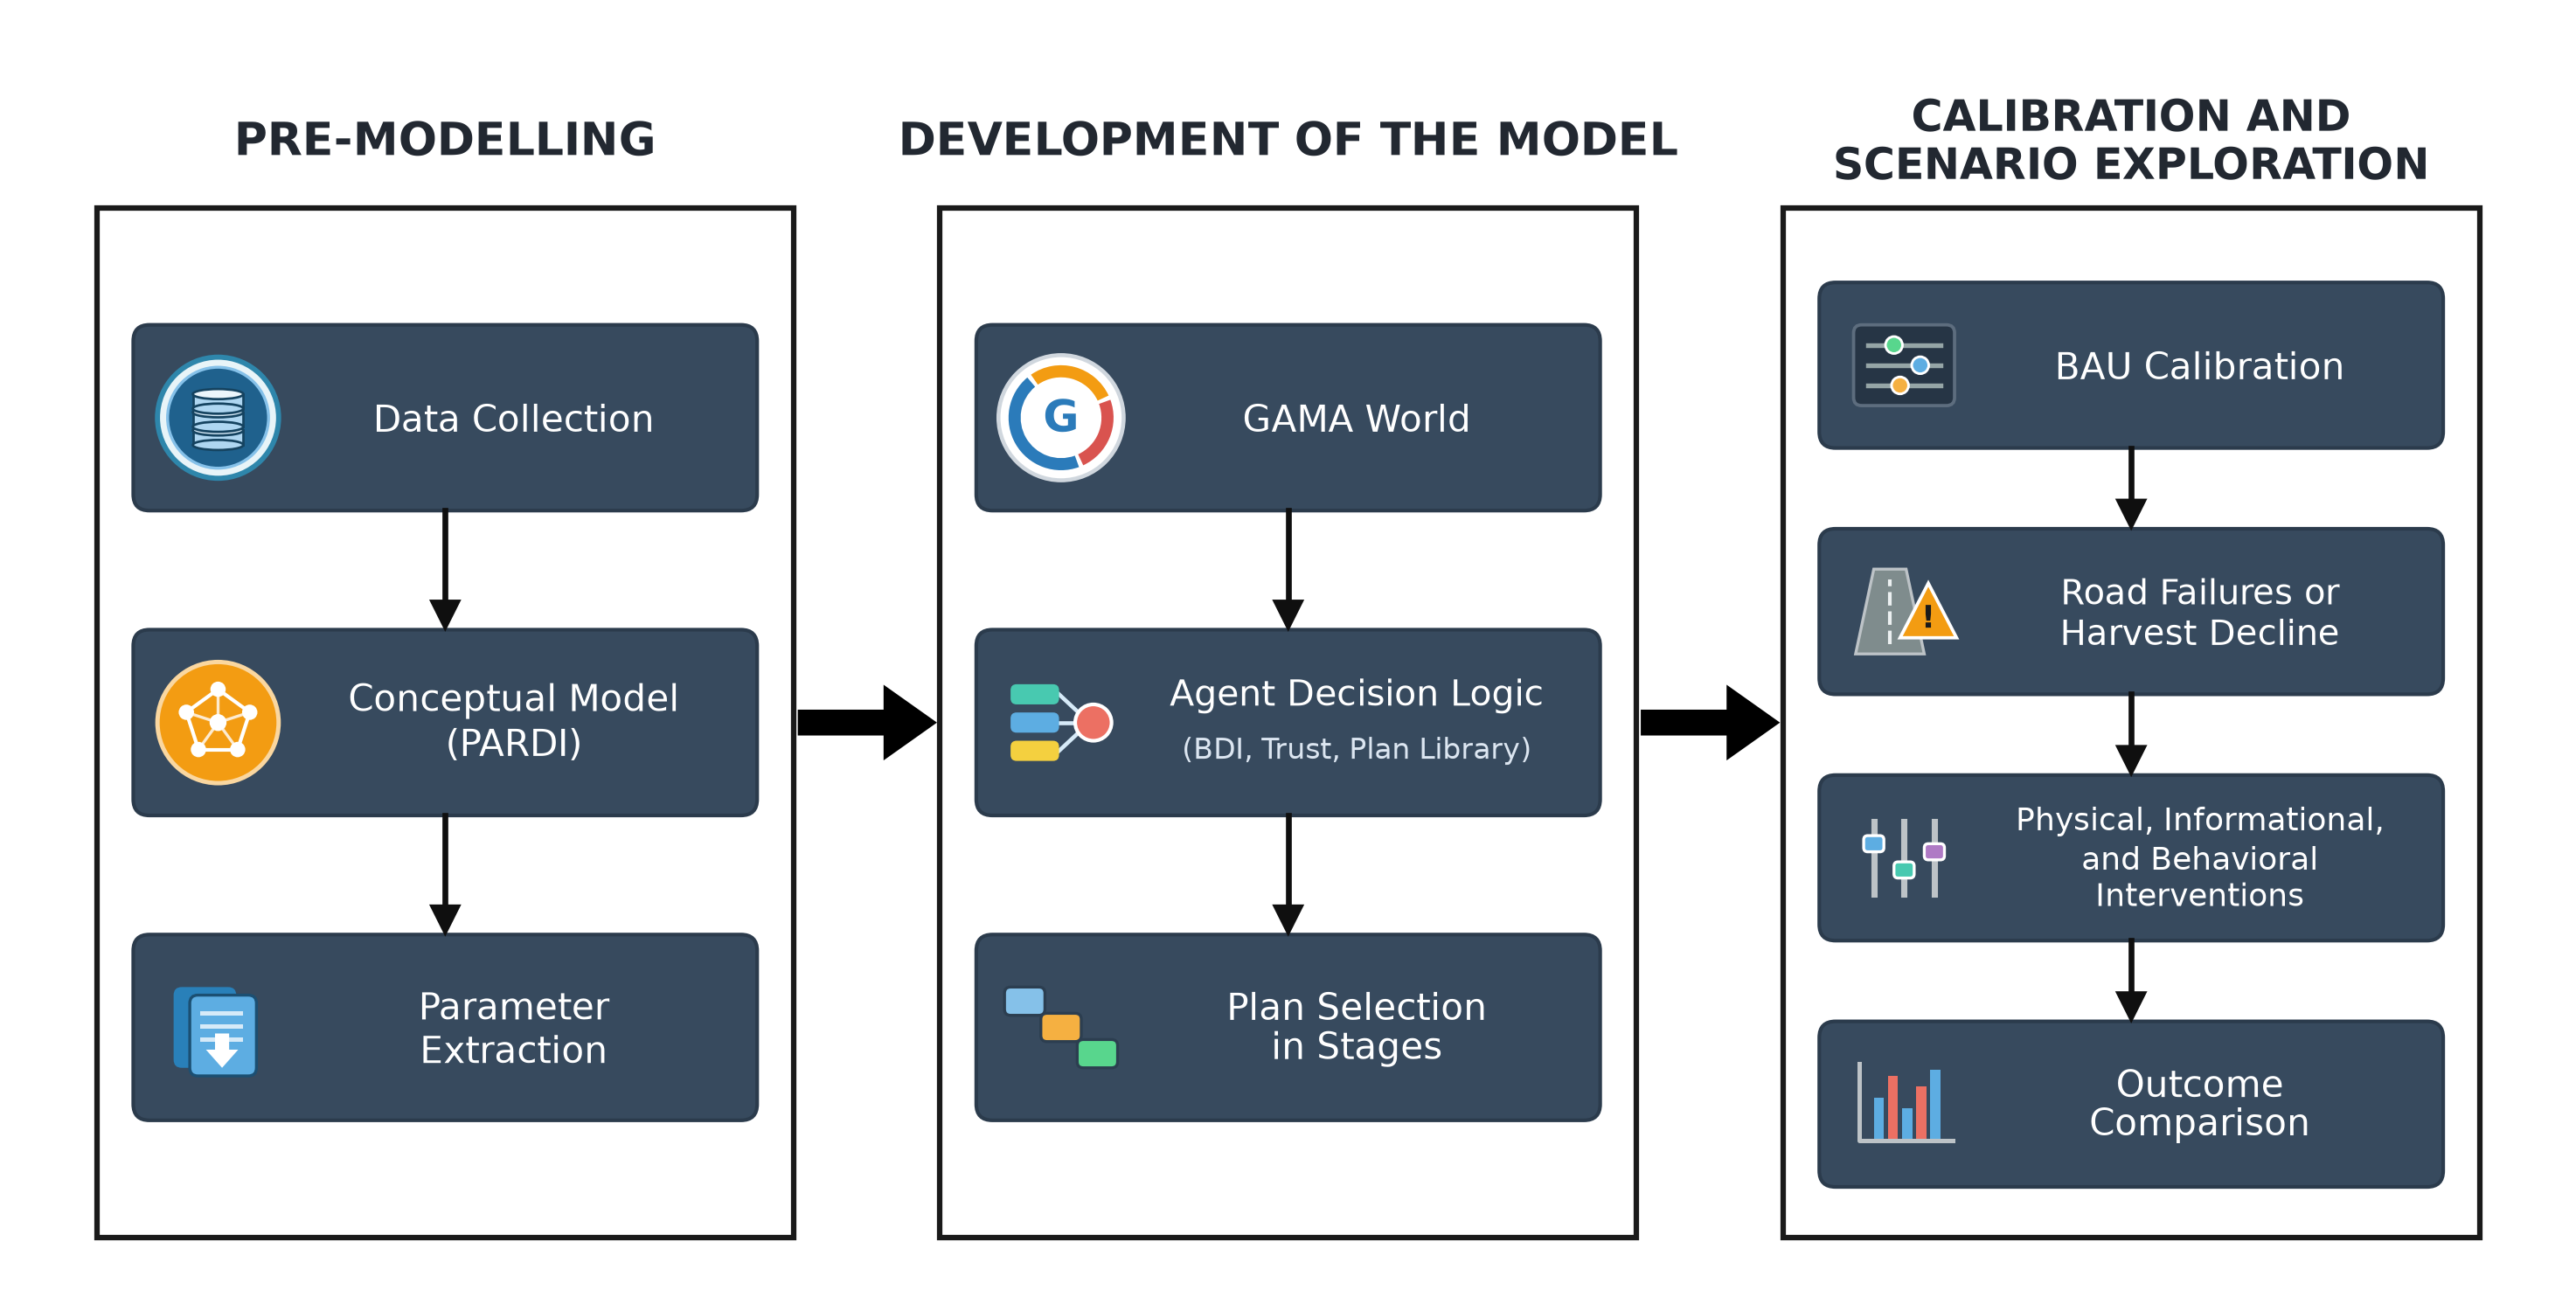
\includegraphics[width=\linewidth]{figures/fig_study_workflow}
				\caption{Methodology: study workflow from data and the conceptual model to scenario evaluation. Stage A assembles the saved data and the PARDI conceptual model. Stage B builds the simulation world, the decision architecture, and staged plan selection. Stage C calibrates business as usual and compares scenarios.}
				\label{fig:ch3-workflow}
			\end{figure}

			Stage A compiles the empirical record: Philippine Statistics Authority (PSA) OpenSTAT tables, the AgriTrakPH compilation of Benguet Agri-Pinoy Trading Center (BAPTC) postings, and OpenStreetMap extracts saved as of 2~September~2026; the Department of Public Works and Highways (DPWH) national-road file (Freedom of Information, 9~October~2026); Department of Agriculture (DA) completed farm-to-market road (FMR) shapefiles (22~October~2026); \citet{deGuzmanBambicoBaconguis2023}; and the documented closures from Chapter~1. Evidence for individual plan rules derives from a targeted literature search as of 24~October~2026. Cleared tickets, named trading pairs, and measured spoilage rates are absent from the public record and excluded from extraction.

			Stage B places seven municipal farm clusters onto a unified road network combining official DPWH highways, Benguet completed FMR segments, and OpenStreetMap local connector roads, with BAPTC as the sole simulated trading post. Inventories, an assumed spoilage process, and harvest schedules run alongside BDI stores, partner and information-source trust, and a fixed plan library. Teacher choices train a multilayer perceptron selector for large-scale runs, evaluated against gradient-boosted trees \citep{Grinsztajn2022}.

			Stage C calibrates business as usual first (starting with cabbage) and then evaluates Scenarios A and B on common random seeds. Across the workflow, closure durations enter as scenario inputs, counterparties are synthetic pairs drawn from published partner-count distributions, and agent decisions are grounded in simulation state and calibrated series rather than language-model pretraining.

			\begingroup
			\setstretch{1}
			\footnotesize
			\setlength{\LTcapwidth}{\textwidth}
			\setlength{\tabcolsep}{3pt}
			\renewcommand{\arraystretch}{1.12}
			\begin{longtable}[l]{@{}>{\raggedright\arraybackslash}p{0.16\textwidth}>{\raggedright\arraybackslash}p{0.20\textwidth}>{\raggedright\arraybackslash}p{0.57\textwidth}@{}}
			\caption{Methodology: study workflow from data and the conceptual model to scenario evaluation. Parameter extraction feeds the simulation world. Decision logs and the runnable world feed calibration.}
			\label{tab:ch3-workflow}\\
			\hline\hline
			Stage & Step & Content \\
			\hline
			\endfirsthead
			\caption[]{Methodology: study workflow from data and the conceptual model to scenario evaluation (continued).}\\
			\hline\hline
			Stage & Step & Content \\
			\hline
			\endhead
			\hline
			\endfoot
			\hline\hline
			\endlastfoot
			A: Pre-modelling & Data collection & PSA OpenSTAT, BAPTC posted prices (via AgriTrakPH), and OpenStreetMap copies (as of 2~September~2026); DPWH national-road file (FOI, 9~October~2026); DA completed farm-to-market road shapefiles (22~October~2026); \citet{deGuzmanBambicoBaconguis2023}; named closure records (Chapter~1) \\
			 & PARDI conceptual model & Researcher-built conceptual model \\
			 & Parameter extraction & Price and production targets; counts of trading partners; hired-haul cost; Ompong travel times; time-step length; evidence for plan rules \\
			B: Development of the model & GAMA world & DPWH corridor clip, Benguet completed farm-to-market segments, and OpenStreetMap local connector roads; seven municipal farm clusters; BAPTC as the only simulated post \\
			 & BDI, trust, and plan library & Belief, desire, and intention stores; partner and information-source trust; a fixed library of plans selected at runtime from that library only \\
			 & Plan selection in stages & A feasible intention continues. The heuristic selects only a unique eligible match. The teacher chooses only among two or more eligible plans. That residual trains the distilled selector (multilayer perceptron; gradient-boosted trees as the baseline) \\
			C: Calibration and scenario exploration & Business-as-usual calibration & Cabbage first; window 27~October~2024--21~December~2025, nominal pesos; PSA farmgate, wholesale, and Baguio retail; Benguet production; BAPTC band is an input and a placement check \\
			 & Scenario A & Ompong 2018 Halsema travel-time multiplier on the calibrated model; replanning minus held commitment on the five outcomes \\
			 & Scenario B & Same shock and seeds. One factor at a time, then a cross, only where the held-commitment arm shows that choices move the outcome \\
			 & Outcome comparison & Evaluated after the monthly price and production baseline is matched \\
			\end{longtable}
			\endgroup

		\subsection{Data and Their Roles}

			Each empirical source is assigned a specific role and scope boundary in the model (Table~\ref{tab:ch3-data}). The PSA, BAPTC (compiled via AgriTrakPH), and OpenStreetMap files on disk are local copies as of 2~September~2026. Among the four study crops, the BAPTC dataset records grade-specific minimum and maximum wholesale prices for cabbage (Wonderball, Rareball, and Scorpio), potato (Granola and LBR), carrot, and chayote.

			The simulated road layer combines the official DPWH clip, the Benguet completed FMR segments, and OpenStreetMap secondary and tertiary local roads, following the data inventory as of 29~October~2026. OpenStreetMap also supplies the named trading-post points.

			\begingroup
			\setstretch{1}
			\footnotesize
			\setlength{\LTcapwidth}{\textwidth}
			\setlength{\tabcolsep}{3pt}
			\renewcommand{\arraystretch}{1.12}
			\begin{longtable}[l]{@{}>{\raggedright\arraybackslash}p{0.24\textwidth}>{\raggedright\arraybackslash}p{0.30\textwidth}>{\raggedright\arraybackslash}p{0.19\textwidth}>{\raggedright\arraybackslash}p{0.20\textwidth}@{}}
			\caption{Methodology: data sources, status, time interval, and role in the model.}
			\label{tab:ch3-data}\\
			\hline\hline
			Series & Status & Time interval & Role \\
			\hline
			\endfirsthead
			\caption[]{Methodology: data sources, status, time interval, and role in the model (continued).}\\
			\hline\hline
			Series & Status & Time interval & Role \\
			\hline
			\endhead
			\hline
			\endfoot
			\hline\hline
			\endlastfoot
			PSA farmgate prices & As of 2~September~2026 & Monthly file, 2010--2026. Fit window 27~October~2024--21~December~2025, nominal pesos & Calibration target in the fit window. Months from 2010 through 2023 are a seasonal-shape check \\
			PSA wholesale prices & As of 2~September~2026 & Monthly file, 2010--2026. Fit window 27~October~2024--21~December~2025, nominal pesos & Calibration target in the fit window. Months from 2010 through 2023 are a seasonal-shape check \\
			PSA Baguio retail prices & As of 2~September~2026 & Monthly file, 2018--2026. Fit window 27~October~2024--21~December~2025, nominal pesos & Calibration target in the fit window. Months from 2018 through 2023 are a seasonal-shape check \\
			PSA Benguet production & As of 2~September~2026 & Quarter, semester, and year, 2010--2026. Error uses the period published inside the fit window & Calibration target at that grain. Earlier periods are a seasonal-shape check \\
			PSA area planted & As of 2~September~2026 & Same periods as production & Sets planted area, which scales supply \\
			BAPTC posted minimum and maximum \citep{AgriTrakPH2025} & Compiled via AgriTrakPH as of 2~September~2026; 19,284 records, 401 dates, 27~October~2024 to 21~December~2025 & Daily; constant across the 24 steps of a day with a record; 20 of 421 calendar days have no record & Exogenous posted band. Check that the simulated minimum and maximum sit on the compiled band \\
			OpenStreetMap roads and named posts & As of 2~September~2026 & Geometry & Local connector roads (secondary and tertiary) and post points; not official FMR attribution \\
			DPWH national roads & On disk; FOI 9~October~2026 & Geometry & Highway layer for the corridor clip \\
			DA completed FMR segments, Benguet & On disk 22~October~2026; 182 segments, 95.6~km & Geometry & Farm-to-highway layer; 40~m snap; no synthetic bridges \\
			Provisional Atok edge & Excluded 22~October~2026 & Geometry, unused & Not used in the model \\
			Geoportal DA FMR preview \citep{GeoportalDAFMR2026} & Viewer check 21~October~2026; not downloadable & Preview & Existence evidence for an Atok corridor \\
			Municipal boundary polygons & On disk 22~October~2026 & Polygons & Map boundaries; not farm locations \\
			\citet{deGuzmanBambicoBaconguis2023} & In hand & Cross-section: 39 farmers, 36 traders & Sets roles, partner counts, information channels, and the haul-cost range \\
			Named road closures & Cited (Chapter~1) & Event narratives & Scenario inputs on the calibrated model; not a validation series \\
			Spoilage, truck capacity, haul cost & Cited shape and order of magnitude \citep{Antolin2024,Fernandez2004,Launio2022,deGuzmanBambicoBaconguis2023} & Not series & Assumptions; swept in sensitivity \\
			Evidence for plan rules & Targeted, non-systematic search as of 24~October~2026 \citep{Antolin2024,Fernandez2004,Launio2022,Nurlina2024,Colon2021,Aghaie2019} & Not series & Related studies used to set plan rules \\
			Destination mix & Maslan (2004), as cited in \citet{Fangasan2009} & Dated structural split & Sets aggregated demand \\
			\end{longtable}
			\endgroup

			The public record leaves LTVTP volumes, named buyers, cleared tickets, measured spoilage, a DPWH event log, a live BAPTC feed, and individual farm coordinates unobserved. These quantities remain outside calibration and validation. Posted ranges are treated as floor and ceiling announcements in the sense of \citet{deGuzmanBambicoBaconguis2023} rather than cleared transaction prices, and trading pairs are synthetic.

		\subsection{Conceptual Model}

			The PARDI frame \citep{Etienne2016} organizes the conceptual model into five components: problematic situation, actors, resources, dynamics, and interactions.

			\subsubsection{Problematic Situation}

			Locally rational choices can propagate the Ompong lengthening of Halsema travel time through the Benguet corridor as delay, isolation, spoilage, price changes, and unmet demand without a concurrent yield shock. Because farmers, traders, truckers, wholesalers, and retailers decide from a partial view, official aggregate series cannot recover who delayed harvest, cancelled trips, held inventory, or raised markups; this mechanism is instead isolated through the held-commitment contrast once baseline prices and production are matched.

			\subsubsection{Actors}

			Five decision-making classes populate the model: the farmer, represented as a municipal cluster and often hauling the lot; the disposer-trader, with the optional financier role folded into that class; the trucker; the wholesaler; and the retailer in Baguio. Cooperatives and associations enter only as information sources. Trading posts are locations rather than decision-makers; BAPTC is the single simulated post (with disposers, wholesalers, and purchasers operating there), while LTVTP and Hangar Market remain cited for corridor structure. Downstream demand is an aggregate load and not an additional decision-making class.

			\subsubsection{Resources}

			The world carries four crops (cabbage, carrot, potato, and chayote; wombok is excluded), inventories along the corridor, and posted prices. At BAPTC, the day's posted minimum and maximum are exogenous and constant across the 24 steps of that day. A disposer ask and a wholesaler markup are chosen inside that band, the retail price equals the ask times 1.35, and the farmgate price is the price on an accepted farmer--disposer lot. PSA farmgate, wholesale, and Baguio retail remain monthly comparison series rather than hourly agent inputs. Road capacity and travel time are defined on Halsema, Kennon Road, Marcos Highway, Naguilian Road, Benguet completed FMR segments, and OpenStreetMap local connector roads. A farmer desire for cash within one to two days reflects slow payment reported for some buyers and enters as a model assumption. Partner trust and information-source trust complete the resource set as unobserved scores per pair.

			\subsubsection{Dynamics}

			Spoilage pressure rises with delay \citep{Antolin2024,Fernandez2004}, with its functional form fixed during calibration and varied in sensitivity analysis. Harvest windows follow the cited crop calendar of potato in March--June, cabbage in July--October, and carrot in November--February (Reyes et al., 2017, as cited in \citealp{deGuzmanBambicoBaconguis2023}), with chayote timing carried as an assumption. The primary shock applies the Ompong 2018 Halsema travel-time multiplier after baseline calibration, with August 2026 retained as an additional case. Intention persistence commits a selected plan across time steps until success, failure, or an explicit drop; in the held-commitment arm of Scenario A, drop rules and reselection remain disabled after the shock begins.

			\subsubsection{Interactions}

			Trading follows the published pattern of \emph{suki} partners, where most farmers named one or two disposers and traders named larger partner sets \citep{deGuzmanBambicoBaconguis2023}. Simulated pairs use that degree distribution with synthetic identifiers. Agents evaluate the posted band against the outcome of the last completed or failed transaction with their usual partner. Because the documented 08:30 and 15:00 announcements apply to LTVTP and no equivalent clock is reported for BAPTC, those hours are not imposed as the BAPTC posting schedule. Route choice relies on the links an agent believes are open, while partner trust and source trust filter the plan library prior to deliberation.

		\subsection{Temporal Resolution}

			One simulation step equals one hour of corridor time, the coarsest resolution at which the Ompong travel-time contrast, a multi-day queue, and a daily posted band remain distinct while still aggregating cleanly to official monthly and periodic series.

			On an hourly step, the ordinary Halsema trip from Buguias to La Trinidad (about three hours) occupies roughly three steps, whereas the Ompong delay (four or five hours) occupies four or five steps \citep{PNA2018,Espiritu2018}; a half-day or daily step would collapse both trips into a single bin and erase that contrast. A queue of two days and two nights spans successive hourly steps \citep{AntonioDumlao2026}, and a daily posted band aggregates 24 hourly steps for comparison with the BAPTC series only on completed days. Table~\ref{tab:ch3-time} maps the empirical clocks onto hourly steps.

			\begingroup
			\setstretch{1}
			\footnotesize
			\setlength{\LTcapwidth}{\textwidth}
			\setlength{\tabcolsep}{3pt}
			\renewcommand{\arraystretch}{1.12}
			\begin{longtable}[l]{@{}>{\raggedright\arraybackslash}p{0.27\textwidth}>{\raggedright\arraybackslash}p{0.21\textwidth}>{\raggedright\arraybackslash}p{0.30\textwidth}>{\raggedright\arraybackslash}p{0.15\textwidth}@{}}
			\caption{Methodology: clocks already in the record, expressed as time steps at one step per hour.}
			\label{tab:ch3-time}\\
			\hline\hline
			Real-world quantity & Source & Time steps at one hour & Role \\
			\hline
			\endfirsthead
			\caption[]{Methodology: clocks already in the record, expressed as time steps at one step per hour (continued).}\\
			\hline\hline
			Real-world quantity & Source & Time steps at one hour & Role \\
			\hline
			\endhead
			\hline
			\endfoot
			\hline\hline
			\endlastfoot
			PSA farmgate, wholesale, and Baguio retail prices & PSA OpenSTAT, as of 2~September~2026 & Hours in that calendar month; aggregate simulated hours to the month before comparison & Calibration target inside 27~October~2024--21~December~2025, nominal pesos \\
			PSA Benguet production & PSA OpenSTAT; quarter, semester, and annual periods & Hours in that period; aggregate to that quarter, semester, or year & Calibration target at the published grain inside the fit window \\
			BAPTC posted minimum and maximum & Compiled via AgriTrakPH, 27~October~2024 to 21~December~2025 & 24 steps per calendar day with a compiled record; the minimum and maximum are constant across those steps & Exogenous band. Placement check only \\
			LTVTP floor and ceiling at 08:30 and 15:00 & \citet{deGuzmanBambicoBaconguis2023} & Not applied to the simulated post & Cited fact, post not simulated \\
			Halsema, Buguias to La Trinidad, about three hours & \citet{PNA2018,Espiritu2018} & About 3 steps & Ordinary travel time \\
			Halsema after Ompong, four or five hours & \citet{PNA2018,Espiritu2018} & 4 or 5 steps & First shock \\
			August 2026 queue of two days and two nights & \citet{AntonioDumlao2026} & Two days and two nights of hourly steps; exact hour count unknown & Additional case; not the first shock \\
			Farmer cash timing of about 1 to 2 days & \citet{deGuzmanBambicoBaconguis2023} & About 24--48 steps & Assumption \\
			Crop calendar: potato March--June, cabbage July--October, carrot November--February & Reyes et al.\ (2017), as cited in \citet{deGuzmanBambicoBaconguis2023} & Hours in those months, applied as month blocks & Assumption (cited schedule) \\
			Spoilage rate and truck capacity & \citet{Antolin2024,Fernandez2004} & Sensitivity defaults (0.002 per hour; 5,000~kg) & Assumption (not calibrated) \\
			Intention persistence & Commitment rule of the architecture & A committed plan lasts across steps until success, failure, or an explicit drop & Assumption (rule) \\
			\end{longtable}
			\endgroup

			Because hourly simulated prices and monthly PSA means represent different temporal intervals, model calibration aggregates hourly outputs to the matching official interval before computing error.

		\subsection{The Simulation World}

			The simulated geography is the Benguet corridor. The highway layer is the official DPWH clip of Halsema, Kennon, Marcos, and Naguilian, plus the alternate connectors reserved for Scenario B. The farm-to-market layer comprises the official Benguet completed FMR segments: 182 polylines and 95.6~km of geometry, with a median segment of about 0.51~km. Direct contact between those segments and the highway is sparse. Measured on 22~October~2026, 15 of 182 segment endpoints lie within 40~m of the highway clip, 34 within 200~m, and 99 within 1~km. OpenStreetMap secondary and tertiary roads in the map crop, including unclassified, residential, and track ways, therefore serve as the connector layer. Farm clusters and completed FMR segments join the highways over those existing local roads. Edges merge at a 40~m snap, and no synthetic bridges are added. A provisional Atok edge aligned with the Philippine Geoportal farm-to-market preview of 21~October~2026 is excluded, because that centerline is absent from the completed-project shapefile \citep{GeoportalDAFMR2026}. Farm agents are seven municipal clusters: Buguias, Mankayan, Atok, Tublay, Kabayan, Bakun, and La Trinidad. Individual farm points are omitted. The merged network places all seven clusters and the post on a single connected component. This merged graph is the cleaned road network.

			BAPTC is the single simulated trading post. LTVTP and Hangar Market remain cited for corridor structure. Demand in the first model is an inelastic daily quantity. The local target is Baguio retail scaled to the PSA retail layer. The outbound target is an aggregate load, including Greater Manila, taken from the dated Maslan split after renormalization. Maslan (2004), as cited in \citet{Fangasan2009}, reports first destinations of 66.24\% to LTVTP, 31.76\% to Hangar Market, 3.50\% to other local Cordillera outlets, and 2\% to Region II. Those four shares sum to 103.5\%. They are not used as printed. The three in-corridor shares sum to 101.5\% and renormalize to 65.26\% for LTVTP, 31.29\% for Hangar Market, and 3.45\% for other Cordillera outlets. The 2\% Region II share remains part of the printed sum and is not a simulated destination. About 48.9\% of farm output continued to Greater Manila. That figure is a separate outbound fraction of farm output, and it sets the outbound daily target. The split records an earlier structure. It is not a 2026 census. The unmet residual of each daily target is counted and cancelled at the end of the day. A price increase under this inelastic demand, with no import response, is an upper illustration.

			The world carries four crops, per-lot inventories, an assumed spoilage process, truck capacity, and harvest schedules. Spoilage pressure rises with delay: measured carrot losses on the Buguias-to-Balintawak path were 0.97\% at harvest, 1.89\% after one day, 35.4\% at five to six days, and 44.55\% at seven to eight days \citep{Antolin2024}, while Cordillera farmer-reported postproduction losses averaged about 12.6\% for cabbage, 10.0\% for carrot, and 13.8\% for potato \citep{Fernandez2004}. Because those studies do not fix an hourly decay rate, spoilage rate and related operational parameters enter as sensitivity assumptions with defaults of 0.002 per hour, a 5,000~kg truck capacity (roughly a six-wheeler), and a hired-haul cost of PHP 3.5 per kg at the midpoint of the published PHP 2 to 5 per kg range \citep{deGuzmanBambicoBaconguis2023}. Posted prices, asks, markups, the 1.35 retail factor, and farmgate pricing follow the resource specification above; Manila retail prices of two to three times Benguet farm receipts support a non-zero marketing margin \citep{Launio2022} without fixing the 1.35 factor.

			Each simulation step runs the following loop:

			\begin{enumerate}
				\item World update advances inventories, spoilage, travel, prices, and any scheduled shock.
				\item Perception updates each agent's beliefs from local observation and messages, with conflicting signals weighted by information-source trust.
				\item Trust update revises partner and source scores after the last completed or failed interaction.
				\item Desire maintenance keeps or revises goals under current pressure.
				\item Deliberation keeps a feasible intention; otherwise it follows staged plan selection.
				\item Intention commits the chosen plan until it succeeds, fails, or is dropped under an explicit condition.
				\item Action executes the intention, and the logger stores beliefs, desires, trust, the plan, and the action for validation and distillation.
			\end{enumerate}

		\subsection{Agent Decision Architecture}

			Every decision-making agent keeps explicit belief, desire, and intention stores, following the practical-reasoning split of \citet{RaoGeorgeff1995}. Implemented as explicit perceive, maintain, deliberate, and act attributes, BDI provides an inspectable computational architecture for local reasoning \citep{WooldridgeJennings1995,MacalNorth2010} rather than a psychological claim about how farmers or traders deliberate.

			Beliefs, desires, intentions, and the plan library are instantiated for the five decision-making classes (Tables~\ref{tab:ch3-mental} and~\ref{tab:ch3-plans}). A farmer's beliefs hold local inventory, location, last cleared price, and trust-weighted signals; desires rank avoiding spoilage, obtaining revenue, fulfilling a standing relationship, and keeping a usual partner; and the intention holds one library plan with its quantity, price band, route, and counterpart. The architecture relies on commitment rules rather than lookahead search or online policy learning. Across steps, agents update beliefs from perception, revise exponential-moving-average trust after success or failure, re-rank desires under spoilage, cash, and unmet-order pressures, and drop intentions only under explicit rules. As boundedly rational actors operating on a partial view, agents face a design trade-off in those drop rules: thresholds that are too strict produce stubborn persistence, whereas thresholds that are too loose collapse the architecture into reactive scripts.

			\begingroup
			\setstretch{1}
			\footnotesize
			\setlength{\LTcapwidth}{\textwidth}
			\setlength{\tabcolsep}{3pt}
			\renewcommand{\arraystretch}{1.12}
			\begin{longtable}[l]{@{}>{\raggedright\arraybackslash}p{0.14\textwidth}>{\raggedright\arraybackslash}p{0.45\textwidth}>{\raggedright\arraybackslash}p{0.34\textwidth}@{}}
			\caption{Methodology: mental-state stores of each decision-making agent.}
			\label{tab:ch3-mental}\\
			\hline\hline
			Store & Contents & Update rule \\
			\hline
			\endfirsthead
			\caption[]{Methodology: mental-state stores of each decision-making agent (continued).}\\
			\hline\hline
			Store & Contents & Update rule \\
			\hline
			\endhead
			\hline
			\endfoot
			\hline\hline
			\endlastfoot
			Beliefs & Local facts (inventory, location, last cleared price) and trust-weighted signals (believed road status, the posted band, and the outcome of the last transaction with a counterpart) & Perception each step; conflicting signals fused by information-source trust \\
			Desires & Ranked goals: avoid spoilage, obtain revenue, fulfill a standing relationship, keep a usual partner & Generated from role and current pressure (spoilage timer, unmet order, low cash) \\
			Intentions & One committed plan with parameters (quantity, price band, route, counterpart) & Persist until success, failure, or an explicit drop condition \\
			Plans & A fixed library of five to eight plans per role & Selected by heuristic BDI, the teacher, or the distilled selector; never invented at runtime \\
			\end{longtable}
			\endgroup

			Commitment is enforced. An intention remains active across steps until it succeeds, fails, or is dropped. Drop conditions are explicit: a confirmed closure on the intended route, counterpart trust falling below a threshold, spoilage risk exceeding a bound, or a higher-priority desire becoming infeasible under current beliefs. The language model cannot silently abandon a committed plan. When the teacher is called, it may only propose a drop or a replacement, and BDI accepts or rejects that proposal against those conditions. Without that commitment, the design would reduce to reactive scripts.

		\subsection{Trust Model}

			Trust is a subsystem of the decision architecture. Two scores are stored per agent. Partner trust \(T_{ij}\) is the directed score of agent \(i\) toward a counterpart \(j\). Information-source trust \(S_{i,k}\) is the directed score of agent \(i\) toward a source \(k\): own observation, the posted band, an official road advisory, or the outcome of the last transaction with a usual partner. Both scores remain in \([0,1]\). Ethnicity, cooperative membership, and named \emph{ga-it} membership are omitted as state variables. The first model has no rumor process.

			Partner trust filters the plan table. The default eligible plan for a farmer is the usual disposer, matching the one-to-two-member networks in the published sample \citep{deGuzmanBambicoBaconguis2023}. If the usual counterpart fails, is unreachable, or repeatedly delays, \(T_{ij}\) falls and the switch plan can become eligible under the Greedy filter. A disposer can reject a lot, and a farmer can wait for the usual buyer, when trust in the alternative is low. Source trust fuses conflicting signals. When observation, the posted band, an official advisory, and the last transaction outcome disagree, the believed predicate is the trust-weighted result rather than the true world state. In the published sample, 85\% of farmers obtained price information from local trading areas and associations, so the posted band sits in the high-trust source set for prices. Official advisories sit in the high-to-medium set for roads. The posted band and the official road advisory each arrive with a lag. High trust in the official advisory, together with a long lag, can leave an agent on a stale road belief. Partner information is the outcome of the last completed or failed transaction with that counterpart, written into the partner-trust update.

			After each completed or failed interaction, partner trust toward that counterpart moves by one exponential moving average for all roles: \(T \leftarrow (1-\alpha)\,T + \alpha \cdot outcome\), with \(outcome\) equal to 1 on success and 0 on failure. The global rate \(\alpha\) is frozen during the business-as-usual fit and is swept later. A source whose claim later matches the observed state is reinforced. A source whose claim is contradicted is discounted. Unused ties decay slowly toward their starting value.

			Because public data do not name farmer--trader pairs, simulated identifiers are arbitrary, and partner trust is initialized from published network structure. Most farmers start with one or two eligible disposers: 46\% of the published farmer sample named one trader, 41\% named two, and 13\% named three to five. Disposers start with a larger usual set: half of the trader sample named one to five \emph{suki} partners, and the rest named six or more. Strangers begin at low-to-moderate trust, which can rise after successful payment and delivery. Unpaid purchaser debts, recorded at PHP 27 million in 2017 and attributed mostly to lowland buyers, explain why farmers discount strangers, and the reported response to cheating is to stop transacting with that person \citep{deGuzmanBambicoBaconguis2023}. These starting values are assumptions informed by that monograph. They are not measured scores for simulated individuals.

		\subsection{Plan Libraries and Response Styles}

			Each role holds a small fixed library of five to eight plans (Table~\ref{tab:ch3-plans}). Selection draws only from that library. Resource constraints, active intentions, and trust filters remove entries before deliberation, and the remainder is the eligible set. The farmer library encodes the documented local moves: harvest or wait, sell to the usual disposer, delay a sale on a low believed price, split a harvest across deliveries, and switch disposer only when the usual counterpart is blocked \citep{deGuzmanBambicoBaconguis2023}. Threshold delay of a sale also has an agent-based analog in a shallot market, where farmers postpone sales below a profit threshold \citep{Nurlina2024}. The trucker plans encode rerouting and delay under disruption, a mechanism with precedent in transport-criticality agent-based models \citep{Colon2021}.

			\begingroup
			\setstretch{1}
			\footnotesize
			\setlength{\LTcapwidth}{\textwidth}
			\setlength{\tabcolsep}{3pt}
			\renewcommand{\arraystretch}{1.12}
			\begin{longtable}[l]{@{}>{\raggedright\arraybackslash}p{0.13\textwidth}>{\raggedright\arraybackslash}p{0.28\textwidth}>{\raggedright\arraybackslash}p{0.52\textwidth}@{}}
			\caption{Methodology: fixed plan libraries by role. Resource constraints, active intentions, trust filters, and the response style remove entries before deliberation.}
			\label{tab:ch3-plans}\\
			\hline\hline
			Role & Plan & Function \\
			\hline
			\endfirsthead
			\caption[]{Methodology: fixed plan libraries by role (continued).}\\
			\hline\hline
			Role & Plan & Function \\
			\hline
			\endhead
			\hline
			\endfoot
			\hline\hline
			\endlastfoot
			Farmer & \texttt{harvest\_now} & Cut ready lots of in-season crops into storage \\
			Farmer & \texttt{wait} & Hold; do not harvest or sell \\
			Farmer & \texttt{sell\_usual\_disposer} & Offer the lot to the usual disposer \\
			Farmer & \texttt{delay\_sale\_low\_price} & Keep the lot when the believed ask is low and spoilage pressure is mild \\
			Farmer & \texttt{split\_deliveries} & Cap the offer at a partial lot against truck capacity \\
			Farmer & \texttt{switch\_disposer\_if\_blocked} & Offer to the next eligible disposer when the usual one is unavailable or trust falls \\
			Disposer (trader) & \texttt{accept\_lot} & Take an inbound farmer lot when buffer room and partner trust allow \\
			Disposer (trader) & \texttt{reject\_lot} & Refuse an inbound lot when the buffer is full or trust is too low \\
			Disposer (trader) & \texttt{ask\_inside\_band} & Choose the ask inside the day's posted minimum and maximum \\
			Disposer (trader) & \texttt{allocate\_usual\_buyer} & Move buffer volume toward the usual wholesaler \\
			Disposer (trader) & \texttt{pay\_after\_clear} & Mark payment cleared after a successful allocation \\
			Trucker & \texttt{route\_halsema} & Prefer Halsema edges on the farm-to-post path \\
			Trucker & \texttt{route\_alternate} & Prefer non-Halsema links when Halsema is believed delayed \\
			Trucker & \texttt{delay\_trip} & Stay idle this step \\
			Trucker & \texttt{partial\_load} & Load only up to capacity \\
			Wholesaler & \texttt{restock} & Pull from disposer buffers when inventory is below target \\
			Wholesaler & \texttt{markup\_inside\_band} & Choose the wholesaler price inside the day's posted band \\
			Wholesaler & \texttt{ration} & Cap outbound volume when inventory is low \\
			Retailer & \texttt{order\_usual} & Order from the usual source while demand is unmet \\
			Retailer & \texttt{set\_retail\_price} & Set the retail price to the ask times 1.35 \\
			Retailer & \texttt{substitute\_skip} & No cross-crop substitution in the first model \\
			\end{longtable}
			\endgroup

			Table~\ref{tab:ch3-plans} is the complete plan library. Response styles filter existing rows for a role or a fraction of agents without adding new plans: Greedy sets \texttt{ask\_inside\_band} and \texttt{markup\_inside\_band} at the top of the band, permits stock holding (farmer \texttt{wait} and \texttt{delay\_sale\_low\_price}, disposer \texttt{reject\_lot}, and trucker \texttt{delay\_trip}), and leaves \texttt{switch\_disposer\_if\_blocked} eligible, whereas Passive keeps \texttt{sell\_usual\_disposer} and \texttt{allocate\_usual\_buyer}, masks switching, and places markups at the low end of the band. The retailer plan \texttt{substitute\_skip} disables cross-crop substitution so unmet demand for one crop is not filled by another. Heterogeneous risk styles under disruption have an agent-based precedent \citep{Aghaie2019}.

		\subsection{Plan Selection in Stages}

			Selection proceeds in a fixed order. A committed intention that remains feasible continues without calling the teacher. If the slot is empty or cleared by a drop rule, the heuristic selects a plan only when one eligible plan uniquely matches the top-ranked desire and its preconditions hold; if the eligible set is empty, the agent waits. When two or more eligible plans remain, the teacher receives a serialized snapshot of current beliefs, active desires, the trust vector, the eligible plans, and the last intention, and returns one structured intention (plan, quantity, price, route, counterpart, and reason code) from that eligible set. Beliefs, desires, and intentions remain in the simulation state rather than the prompt, and a validator rejects any proposal outside the eligible set or below the trust threshold before commitment, logging all rejections. This residual of multi-plan decisions forms the sole teacher and student training distribution.

			Because seven municipal clusters represent individual farms without individual farm coordinates, combining cluster-level representation, the unique-match heuristic, and the distilled selector keeps large Monte Carlo runs tractable. Each residual teacher decision and its snapshot are logged across varied business-as-usual episodes (targeting 10,000 to 100,000 decisions across roles with varying seeds, seasons, demand noise, and minor shocks). On this dataset, I train a per-role multilayer perceptron with a softmax over the plan library (ineligible plans masked) and regression heads for quantity and price, benchmarked against gradient-boosted trees on the same tabular features \citep{Grinsztajn2022}. Training uses behavior cloning with optional soft labels \citep{Hinton2015}, split by episode and shock rather than random steps to prevent leakage across disruption states; a heterogeneous graph model is retained only as an ablation. Candidate selectors are evaluated on plan agreement (also benchmarked against the most frequent eligible plan in the training log), parameter error, rollout calibration drift, and inference time. If surrogate calibration drift exceeds the pre-committed tolerance, disruption runs fall back to the teacher or heuristic rather than relabeling student-visited states.

			Four selection arms are compared on the same world: heuristic BDI, heuristic BDI with trust disabled, BDI with the language-model teacher, and BDI with the distilled selector. Disabling trust removes partner filtering and signal fusion while retaining drop rules and reselection. Together, these arms evaluate whether the heuristic, teacher, and distilled selector produce consistent shock rankings, whereas the held-commitment contrast separates behavioral replanning from the physical travel-time change.

		\subsection{Business-as-Usual Calibration}

			Before evaluating disruptions, business-as-usual conditions are calibrated over 27~October~2024 through 21~December~2025 in nominal pesos as published. Cabbage is fitted first, followed by carrot, potato, and chayote. Calibration targets are monthly PSA farmgate prices, monthly PSA wholesale prices, monthly PSA City of Baguio retail prices, and Benguet production at its published quarter, semester, or annual grain inside the window; earlier PSA observations (2010--2023) serve only as a seasonal-shape check.

			Prior to any disruption run, I report monthly mean absolute percentage error for each PSA price layer by crop and production error at the published reporting grain against tolerances fixed before inspection. The BAPTC check verifies only whether simulated posted minimum and maximum prices fall within the compiled daily band \citep{AgriTrakPH2025}, which covers 401 observation dates across one full rotation of the crop calendar (401 dates for cabbage Wonderball, 400 for potato Granola, 398 for carrot, and 399 for chayote, with 20 of 421 calendar days unrecorded). Because the band is an exogenous input and the compiled series is unofficial and omits cleared prices and corridor throughput, sitting inside the band does not validate the market-clearing mechanism.

			The PSA series and the BAPTC band measure distinct market objects: PSA wholesale reflects provincial or regional commodity prices across the month, whereas BAPTC postings report daily grade-specific floor and ceiling ranges (such as Wonderball or Granola) at a single facility. Moreover, monthly PSA averages smooth over the sub-daily and multi-day dynamics (such as a three-hour versus four-to-five-hour trip or a two-day queue) that Scenario A resolves.

			During calibration, the posted band, road network, crop calendar, partner degrees, spoilage form, truck capacity, haul cost, 1.35 retail factor, and trust-update rate remain fixed for subsequent sensitivity sweeps, while a pre-specified set of supply and demand parameters is adjusted to fit the official targets. If asks and markups constrained within the posted band cannot match the PSA series, the gap is reported directly rather than relaxing the band. Secondary checks verify the 2010--2023 seasonal shape and confirm that simulated farmers transact primarily through one or two usual disposers \citep{deGuzmanBambicoBaconguis2023}. Road-closure hours, LTVTP throughput, and named trading pairs remain excluded from calibration targets.

		\subsection{Validation and Calibration Plan}

			Model validation is structured across six levels:

			\begin{enumerate}
				\item \textbf{Conceptual and structural.} The PARDI diagram is researcher-built from Chapter~1, frozen datasets, and \citet{deGuzmanBambicoBaconguis2023}, with unobserved quantities explicitly labeled as assumptions and withheld from fit targets.
				\item \textbf{Calibration.} Cabbage is fitted first, followed by carrot, potato, and chayote, over 27~October~2024 through 21~December~2025 in nominal pesos. Pre-committed metrics are monthly mean absolute percentage error for PSA farmgate, wholesale, and Baguio retail prices by crop and production error at the published grain, alongside the BAPTC exogenous posted-band check \citep{AgriTrakPH2025}.
				\item \textbf{Behavioral comparison.} Matching business-as-usual prices and production serves as the baseline prerequisite, paired with the structural check that farmers sell mainly through one or two usual disposers \citep{deGuzmanBambicoBaconguis2023}. Behavioral amplification is measured as the difference between replanning and held-commitment runs.
				\item \textbf{Process record.} Decision logs and the four selection arms (heuristic BDI, heuristic BDI without trust, BDI with the teacher, and BDI with the distilled selector) support model inspectability and distillation verification, with illustrative action traces documenting which plans fired rather than claiming equivalence to named farmers.
				\item \textbf{Sensitivity.} Fixed baseline parameters are swept after calibration. Scenario B varies one factor at a time around the Scenario A baseline, standardizes changes by the Scenario A ensemble standard deviation, and crosses influential factor levels on common random seeds for outcomes affected by replanning.
				\item \textbf{Baseline prerequisite.} Disruption scenarios are interpreted only after business-as-usual prices and production are matched.
			\end{enumerate}

		\subsection{Disruption Scenarios}

			Five outcomes are evaluated across scenarios: delay (extra hours on completed farm-to-post trips relative to the baseline origin--destination time), isolation (cluster-days with no believed-open path to BAPTC), spoilage (kilograms lost by crop and location: farm store, in transit, and post), price change (simulated price minus matched baseline price in pesos per kilogram and percent by crop and layer), and unmet demand (daily target minus kilograms delivered by day's end).

			The primary experiment applies the Ompong 2018 travel-time multiplier on Halsema, reflecting reported Buguias-to-La Trinidad travel lengthening from about three hours to four or five hours and causing late trucks to miss buyers \citep{PNA2018,Espiritu2018}. Applied to the 27~October~2024--21~December~2025 calibrated model without a yield shock or severed-road coding, this scenario is not a backcast of 2018 prices. Closure durations enter as fixed scenario inputs. Additional historical events test the same mechanisms as robustness cases: Pepeng 2009 closes Kennon Road, Marcos Highway, and Naguilian Road simultaneously \citep{GMANews2009}; Carina 2024 and July 2025 impose repeated Kennon closures \citep{Rappler2024,PIA2025}; and August 2026 models post queue congestion and spoilage \citep{AntonioDumlao2026}. All runs are counterfactuals under stated assumptions.

			Scenario A compares two arms on identical random seeds after baseline calibration: a replanning arm (with drop rules and reselection active) and a held-commitment arm (holding business-as-usual intentions fixed once the shock starts, while updating travel times on in-progress trips). Behavioral amplification equals the replanning arm minus the held-commitment arm across the five outcomes; any shortage appearing in the held-commitment arm is attributable to the physical travel-time change alone.

			Scenario B retains the same shock and seeds to rank factors on outcomes sensitive to replanning, evaluated one outcome at a time via standardized one-factor-at-a-time contrasts followed by a crossed design over influential levels. The factors are alternate-road capacity, closure duration, posted-band and road-advisory lag, trust in the official advisory, and the share of agents masked by Passive rather than Greedy styles. Disabling trust (removing partner filtering and signal fusion while keeping replanning active) and comparing the four selection arms provide two additional model contrasts.

		% TODO: candidate to move to the Discussion chapter once drafted
		\subsection{Limitations of the Design}

			The model is a stylized agent-based representation anchored to aggregate public price and production series under explicit assumptions. OpenStreetMap local connectors provide open geometry rather than official farm-to-market road attribution, and outflow edges terminate at the boundary of the cleaned road network. Because the baseline match evaluates aggregate series without an interview-based process test, agreement with monthly prices does not verify that teacher reason codes mirror individual farmers' or traders' reasoning. Price increases under inelastic demand and no import response represent upper-bound illustrations, counterparties are synthetic pairs consistent with published degree distributions rather than measured social capital, and language-model decisions rely on generic reasoning grounded in the simulation snapshot and calibrated series rather than corridor-specific pretraining. Unobserved quantities are treated as assumptions and examined through sensitivity analysis, with prompts, plan libraries, seeds, and decision logs versioned alongside every run.
		
		
		\section{RESULTS AND DISCUSSION}
			\lipsum[4]
			
			%TABLE INSERTION SAMPLE
			\begin{table}[ht]
			\vspace{4ex}
			\centering
				\caption{Test Caption Table}
				
				\label{table:Test Caption Table}
				\begin{tabular*}{\textwidth}{@{\extracolsep{\fill}}llllll}
				\hline
				\hline
				1 & 2 & 3 & 4 & 5 & 6 \\ \hline
				1 & 2 & 3 & 4 & 5 & 6 \\
				1 & 2 & 3 & 4 & 5 & 6 \\
				1 & 2 & 3 & 4 & 5 & 6 \\ \hline\hline
				\end{tabular*} 
			\vspace{4ex}
			\end{table}
			
			\lipsum[4-10]
			\lipsum[5]
		
		\section{SUMMARY AND CONCLUSION}
			\lipsum[4]
		
		%References command
		%Parameter is the references bib file without extension
		\makereferences{references}
			
	\end{mainmatter}
\end{document}
